\documentclass{Style}

\begin{document}
\normalfont
\clearpage\thispagestyle{empty}
\setcounter{page}{0}
\vspace*{4.5cm}
\begin{center}
	\begin{tikzpicture}
	\foreach \x in {0,10,...,360}
	\draw [->,line width =2,color={red!70!blue}] (0:0) .. controls (\x + 60:1) .. ( \x :1) .. controls +(\x - 60:1) .. (\x:2) .. controls +(\x+60:1) .. (\x:3) .. controls +(\x - 60:1) .. (\x:4);
	
	\draw[-latex,white,postaction={decorate},decoration={text along path,
		text={HAMIDREZA EBTEHAJ - HAMIDREZA EBTEHAJ - HAMIDREZA EBTEHAJ - HAMIDREZA EBTEHAJ - HAMIDREZA EBTEHAJ - HAMIDREZA EBTEHAJ - Author -},text align=center}]
	(0:0) circle (4.4);
	\end{tikzpicture}
	\begin{equation} 
	P_n = (n-2\lceil\frac{n}{2}\rceil+1)[\theta:\lceil \frac{n}{2}\rceil] + (2\lceil\frac{n}{2}\rceil-n) \big\{P_{n-1} + [\theta + (-1)^n:\lceil \frac{n}{2}\rceil] \big\} \quad \quad , 0 \leqslant \theta < 2\pi , n \in \mathbb{N}
	\end{equation}
\end{center}
\vspace*{\fill}

\tableofcontents

\chapter{\LaTeX \, Reference}
\section{Xcolor}

\begin{note}[{Color Note 1}]\\
How does a mixture of $40\%$ green and $60\%$ yellow look like?\\
(Answer: $40\%$ \tikz \draw[fill=green] (0,0) rectangle (6mm,3mm);
$+ 60\%$ \tikz \draw[fill=yellow] (0,0) rectangle (6mm,3mm);
$=$ \tikz \draw[fill=green!40!yellow] (0,0) rectangle (6mm,3mm);
e.g., \verb|\color{green!40!yellow} |)
\end{note}
\begin{note}[{Color Note 2}]\\
And how does its complementary color look like?\\
 (Answer:  \tikz \draw[fill=-green!40!yellow] (0,0) rectangle (6mm,3mm);
accessible via \verb|\color{-green!40!yellow} |)
\end{note}
\begin{note}[{Color Note 3}]\\
Now mix three parts of last color with two parts of its complement and one part of red, PLZ!:\\
(Answer: $3 \times $ \tikz \draw[fill=-green!40!yellow] (0,0) rectangle (6mm,3mm);
$+ 2 \times$ \tikz \draw[fill=green!40!yellow] (0,0) rectangle (6mm,3mm);
$+ 1 \times$ \tikz \draw[fill=red] (0,0) rectangle (6mm,3mm);
$=$ \tikz \draw[fill={rgb:-green!40!yellow,3;green!40!yellow,2;red,1}] (0,0) rectangle (6mm,3mm);
\\ e.g., \verb|\color{rgb:-green!40!yellow,3;green!40!yellow,2;red,1} |)
\end{note}
\section{Tikz}

\begin{note}[Tiks inline commands]: 
use \textbf{\textbackslash tikz} for simple inline commands
\end{note}
	
\begin{note}[Draw]: \\
use \textbf{\textbackslash draw} to draw a line\\
\verb|\tikz \draw (0pt,0pt) -- (20pt,6pt);|
\tikz \draw (0pt,0pt) -- (20pt,6pt);
\\
\verb|\tikz \draw (0pt,0pt) -- (20pt,0pt);|
\tikz \draw (0pt,0pt) -- (20pt,0pt);
\\
\verb|\tikz \draw (0pt,0pt) -- (0pt,20pt);|
\tikz \draw (0pt,0pt) -- (0pt,20pt);
\end{note}

\begin{note}[\textbackslash fill and \textbackslash circle usage]:\\
	\verb|\tikz \fill[orange] (0,0) circle (1ex);|
	\tikz \fill[orange] (0,0) circle (1ex); 
\end{note}
\begin{note}[Large pictures]:\\
use \textbf{\textbackslash begin\{tikzpivture\}} and \textbf{\textbackslash end\{tikzpicture\}} for larger pictures
\begin{table}[h]
\centering
\begin{tabular}{c|c}
\begin{lstlisting}[language={[LaTeX]TeX},basicstyle=\ttfamily]
\draw[style=dashed] (2,.5) circle (0.5);
\draw[fill=green!50] (1,1)
ellipse (.5 and 1);
\draw[fill=blue] (0,0) rectangle (1,1);
\draw[style=thick]
(3,.5) -- +(30:1) arc(30:80:1) -- cycle;
\end{lstlisting} &
	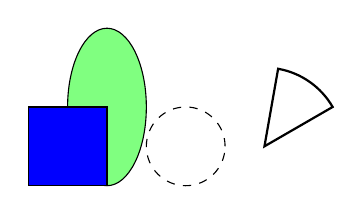
\begin{tikzpicture}
	\draw[style=dashed] (2,.5) circle (0.5);
	\draw[fill=green!50] (1,1)
	ellipse (.5 and 1);
	\draw[fill=blue] (0,0) rectangle (1,1);
	\draw[style=thick]
	(3,.5) -- +(30:1) arc(30:80:1) -- cycle;
	\end{tikzpicture}
\end{tabular}
\end{table}
\end{note}
	
\begin{note}[Cordinate System]:
\begin{itemize}
\item It Starts from lower left
\item To make boundaries visible use :
\begin{lstlisting}
\hspace*{..}, \vspace*{..}
\end{lstlisting}
\item sample:
\begin{lstlisting}
\vspace{-1cm}\hspace{8cm}
\begin{tikzpicture}[ scale=.8, show background rectangle]
\draw (2,2) circle (1);
\draw (0 mm, 0 pt) -- (16 em, 1);
\end{lstlisting}
\vspace{-1cm}\hspace{8cm}
\begin{tikzpicture}[ scale=.8, show background rectangle]
\draw (2,2) circle (1);
\draw (0 mm, 0 pt) -- (16 em, 1);
\end{tikzpicture}
\end{itemize}
\begin{remark}
A solution in the spirit of \LaTeX \, would be the use of a multicolumn environment or of minipages. But sometimes the 
\textbf{\textbackslash hspace \textbackslash vspace} hack is faster and more flexible.)
\end{remark}
\end{note}
	
\begin{note}[Paths]:\\

\begin{tabular}{c l}
\tikz \path[draw] (1,1) -- (2,2) -- (3,1); &
\begin{lstlisting}
\tikz \path[draw] (1,1) -- (2,2) -- (3,1);
\end{lstlisting} \\
\tikz \path[draw,line width=4pt] (1,1) -- (2,2)--(3,1)--cycle; &
\begin{lstlisting}
\tikz \path[draw,line width=4pt] (1,1) -- (2,2)--(3,1)--cycle;
\end{lstlisting} \\
\tikz \path[draw, fill=green!20] (1,1) -- (2,2) -- (3,1) --cycle; &
\begin{lstlisting}
\tikz \path[draw, fill=green!20] (1,1) -- (2,2) -- (3,1) --cycle;
\end{lstlisting} \\
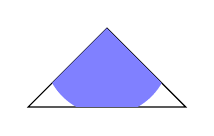
\begin{tikzpicture}
\path[clip, draw] (1,1)--(2,2)--(3,1)--cycle;
\path[fill=blue!50] (2, 1.7) circle (.8);
\end{tikzpicture} &
\begin{lstlisting}
\path[clip, draw] (1,1)--(2,2)--(3,1)--cycle;
\path[fill=blue!50] (2, 1.7) circle (.8);
\end{lstlisting}
\end{tabular}
\end{note}
	
\begin{note}[Shading]:\\
	
	\begin{tabular}{c l}
		\tikz \path[shade,draw] (1,1) -- (2,2)--(3,1)--cycle; &
\begin{lstlisting}
\tikz \path[shade,draw] (1,1) -- (2,2)--(3,1)--cycle;
\end{lstlisting} \\
		\tikz \shade[left color=red] (1,1)--(2,2)--(3,1)--cycle; &
\begin{lstlisting}
\tikz \shade[left color=red] (1,1)--(2,2)--(3,1)--cycle;
\end{lstlisting} \\
		\tikz \shade[top color=red, bottom color=green]
		(0,0) rectangle (2,1); &
\begin{lstlisting}
\tikz \shade[top color=red, bottom color=green]
(0,0) rectangle (2,1);
\end{lstlisting} \\
		\tikz \shade[draw,shading=radial, inner color=blue]
		(0,0) rectangle (2,1); &
\begin{lstlisting}
\tikz \shade[draw,shading=radial, inner color=blue]
(0,0) rectangle (2,1);;
\end{lstlisting} \\
		\tikz \shade[shading=ball, ball color=blue]
		(0,0) rectangle (2,1); &
\begin{lstlisting}
\tikz \shade[shading=ball, ball color=blue]
(0,0) rectangle (2,1);
\end{lstlisting} \\
		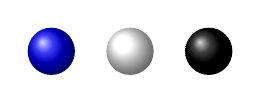
\begin{tikzpicture}
		\shade[shading=ball, ball color=blue] (0,0) circle (.3);
		\shade[shading=ball, ball color=white] (1,0) circle (.3);
		\shade[shading=ball, ball color=black] (2,0) circle (.3);
		\end{tikzpicture} &
\begin{lstlisting}
\shade[shading=ball, ball color=blue] (0,0) circle (.3);
\shade[shading=ball, ball color=white] (1,0) circle (.3);
\shade[shading=ball, ball color=black] (2,0) circle (.3);
\end{lstlisting}
	\end{tabular}
\end{note}
\begin{note}[Polar Coordinates]:\\

\begin{tabular}{c | l}
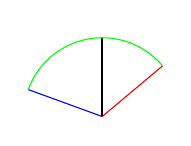
\begin{tikzpicture}
\draw[color=red] (0,0) -- (40:1);
\draw[color=blue] (0,0) -- (160:1);
\draw[thick] (0,0) -- (90:1);
\draw[color=green] (40:1) arc (40:160:1);
\end{tikzpicture} &
\begin{lstlisting}
\draw[color=red] (0,0) -- (40:1);
\draw[color=blue] (0,0) -- (160:1);
\draw[thick] (0,0) -- (90:1);
\draw[color=green] (40:1) arc (40:160:1);
\end{lstlisting}
\end{tabular}
\end{note}
\begin{note}[Curved Lines]:\\

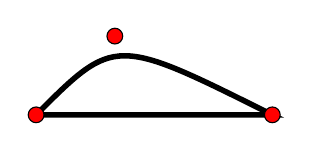
\begin{tikzpicture}
\draw[line width=2pt] (0, 0) .. controls(1,1) .. (3, 0) --cycle;
\draw[fill = red] (0,0) circle (1mm);
\draw[fill = red] (1,1) circle (1mm);
\draw[fill = red] (3,0) circle (1mm);
\end{tikzpicture}
\begin{lstlisting}
\draw[line width=2pt] (0, 0) .. controls(1,1) .. (3, 0) --cycle;
\end{lstlisting} 

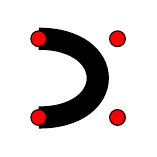
\begin{tikzpicture}
\draw[line width=8pt] (0, 0) ..
controls(1, 0) and (1, 1)
.. (0, 1);
\draw[fill = red] (0,0) circle (1mm);
\draw[fill = red] (1,0) circle (1mm);
\draw[fill = red] (1,1) circle (1mm);
\draw[fill = red] (0,1) circle (1mm);
\end{tikzpicture}
\begin{lstlisting}
\draw[line width=8pt] (0, 0) ..
		controls(1, 0) and (1, 1)
			.. (0, 1);
\end{lstlisting} 

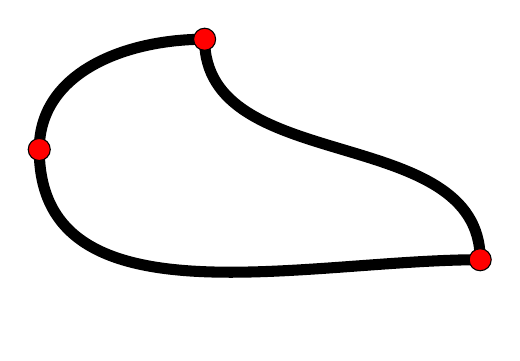
\begin{tikzpicture}[scale=.7]
\draw[line width=4pt] (0,0) to [out=90, in=180] (3,2)
							to [out=-90, in=90] (8,-2)
							to [out=180, in=-90] (0,0);
\draw[fill = red] (0,0) circle (2mm);
\draw[fill = red] (3,2) circle (2mm);
\draw[fill = red] (8,-2) circle (2mm);
\end{tikzpicture}
\begin{lstlisting} [language={[LaTeX]TeX},basicstyle=\ttfamily]
\draw[line width=4pt] (0,0) to [out=90, in=180] (3,2)
				to [out=-90, in=90] (8,-2)
				to [out=180, in=-90] (0,0);
\end{lstlisting} 
\end{note}
\begin{note}[Arrows, Dash patterns]:\\
\begin{tabular}{c l}
\tikz \draw[->] (0,0) -- (1,0); &
\begin{lstlisting} [language={[LaTeX]TeX},basicstyle=\ttfamily]
\tikz \draw[->] (0,0) -- (1,0);
\end{lstlisting} \\

\tikz \draw[dotted, >->>] (0,0) -- (1,0); &
\begin{lstlisting} [language={[LaTeX]TeX},basicstyle=\ttfamily]
\tikz \draw[dotted, >->>] (0,0) -- (1,0);
\end{lstlisting} \\

\tikz \draw[|<->|] (0,0) -- (1,0); &
\begin{lstlisting} [language={[LaTeX]TeX},basicstyle=\ttfamily]
\tikz \draw[|<->|] (0,0) -- (1,0);
\end{lstlisting} \\

\tikz \draw[dashed, o-)] (0,0) -- (1,0); &
\begin{lstlisting} [language={[LaTeX]TeX},basicstyle=\ttfamily]
\tikz \draw[dashed, o-)] (0,0) -- (1,0);
\end{lstlisting} \\

\tikz \draw[loosely dashed] (0,0) -- (1,0); &
\begin{lstlisting} [language={[LaTeX]TeX},basicstyle=\ttfamily]
\tikz \draw[loosely dashed] (0,0) -- (1,0);
\end{lstlisting} \\

\tikz \draw[densely dotted] (0,0) -- (1,0); &
\begin{lstlisting} [language={[LaTeX]TeX},basicstyle=\ttfamily]
\tikz \draw[densely dotted] (0,0) -- (1,0);
\end{lstlisting} \\

\tikz \draw[->] (0,0) .. controls (.2,-.2) .. (1, 0); &
\begin{lstlisting} [language={[LaTeX]TeX},basicstyle=\ttfamily]
\tikz \draw[->] (0,0) .. controls (.2,-.2) .. (1, 0);
\end{lstlisting} \\
\end{tabular}
\end{note}
	
\begin{note}[Clipping and Scope]\\

\begin{itemize}
\item After a \textbf{\textbackslash Clip} Command,all subsequent drawings are clipped, only the parts
inside the clipping region are drawn.
\item Use the \textbf{Scope} environment to restrict the effect of clipping
\end{itemize}

\begin{tabular}{c|l}
	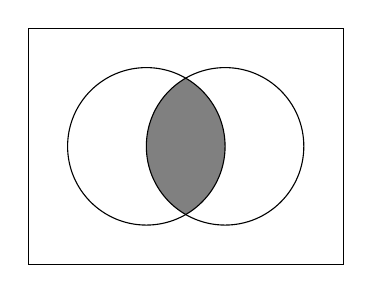
\begin{tikzpicture}
	\draw (-2, 1.5) rectangle (2, -1.5);
	\begin{scope}
	\clip (-0.5, 0) circle (1);
	\clip ( 0.5, 0) circle (1);
	\fill[color=gray] (-2,1.5)
	rectangle (2,-1.5);
	\end{scope}
	\draw (-0.5, 0) circle (1);
	\draw ( 0.5, 0) circle (1);
	\end{tikzpicture} &
\begin{lstlisting} [language={[LaTeX]TeX},basicstyle=\ttfamily]
\draw (-2, 1.5) rectangle (2, -1.5);
\begin{scope}
\clip (-0.5, 0) circle (1);
\clip ( 0.5, 0) circle (1);
\fill[color=gray] (-2,1.5) rectangle (2,-1.5);
\end{scope}
\draw (-0.5, 0) circle (1);
\draw ( 0.5, 0) circle (1);
\end{lstlisting} \\
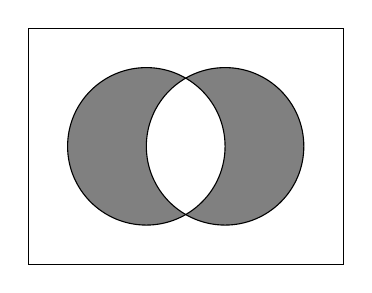
\begin{tikzpicture}
\draw (-2, 1.5) rectangle (2, -1.5);
\fill[color=gray] (-0.5, 0) circle (1);
\fill[color=gray] ( 0.5, 0) circle (1);
\begin{scope}
\clip (-0.5, 0) circle (1);
\clip ( 0.5, 0) circle (1) ;
\draw[fill=white] (-2,1.5)
rectangle (2,-1.5);
\end{scope}
\draw (-0.5, 0) circle (1);
\draw ( 0.5, 0) circle (1);
\end{tikzpicture} &
\begin{lstlisting} [language={[LaTeX]TeX},basicstyle=\ttfamily]
\draw (-2, 1.5) rectangle (2, -1.5);
\fill[color=gray] (-0.5, 0) circle (1);
\fill[color=gray] ( 0.5, 0) circle (1);
\begin{scope}
\clip (-0.5, 0) circle (1);
\clip ( 0.5, 0) circle (1) ;
\draw[fill=white] (-2,1.5) rectangle (2,-1.5);
\end{scope}
\draw (-0.5, 0) circle (1);
\draw ( 0.5, 0) circle (1);
\end{lstlisting} 
\end{tabular}
\end{note}
	
\begin{note}[Nodes]:
\begin{itemize}
\item Nodes are added to paths after the path is drawn:
\tikz \path[draw] (0, 0) node {A} -- (1,0) -- (1,1) node {B};
\begin{lstlisting}[language={[LaTeX]TeX},basicstyle=\ttfamily]
\tikz \path[draw] (0, 0) node {A} -- (1,0) -- (1,1) node {B};
\end{lstlisting}	
\item Nodes can get a name for later references. Nodes have many options.
\begin{tikzpicture}
\path[draw] (0, 0) node[draw] (nodeA) {$A^2$} -- (1,0)
-- (1,1) node[ellipse,fill=green](nodeB) {\tiny B};
\draw[red,->] (nodeA) -- (nodeB);
\end{tikzpicture}
\begin{lstlisting}[language={[LaTeX]TeX},basicstyle=\ttfamily]
\path[draw] (0, 0) node[draw] (nodeA) {$A^2$} -- (1,0)
-- (1,1) node[ellipse,fill=green](nodeB) {\tiny B};
\draw[red,->] (nodeA) -- (nodeB);
\end{lstlisting}

\item Another Sample \\

\begin{tabular}{c l}
\begin{tikzpicture}
\begin{tikzpicture}[scale=.9, transform shape]
\tikzstyle{every node} = [circle, fill=gray!30]
\node (a) at (0, 0) {A};
\node (b) at +(0: 1.5) {B};
\node (c) at +(60: 1.5) {C};
\foreach \from/\to in {a/b, b/c, c/a}
\draw [->] (\from) -- (\to);
\end{tikzpicture}
\end{tikzpicture} &
\begin{lstlisting} [language={[LaTeX]TeX},basicstyle=\ttfamily]
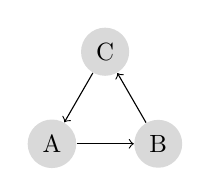
\begin{tikzpicture}[scale=.9, transform shape]
\tikzstyle{every node} = [circle, fill=gray!30]
\node (a) at (0, 0) {A};
\node (b) at +(0: 1.5) {B};
\node (c) at +(60: 1.5) {C};
\foreach \from/\to in {a/b, b/c, c/a}
	\draw [->] (\from) -- (\to);
\end{tikzpicture}
\end{lstlisting} 	
\end{tabular}
\item Nodes on a path can have a placement option\\

\begin{tabular}{c | l}

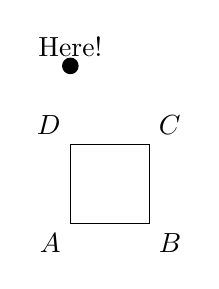
\begin{tikzpicture}
\fill (0,2) circle (3pt) node[above] {Here!};
\draw (0,0) node[below left] {$A$} --
(1,0) node[below right] {$B$} --
(1,1) node[above right] {$C$} --
(0,1) node[above left] {$D$} -- cycle;
\end{tikzpicture} &
\begin{lstlisting} [language={[LaTeX]TeX},basicstyle=\ttfamily]
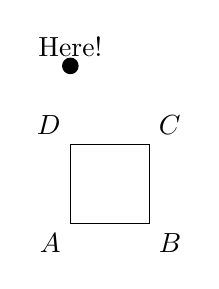
\begin{tikzpicture}
\fill (0,2) circle (3pt) node[above] {Here!};
\draw (0,0) node[below left] {$A$} --
(1,0) node[below right] {$B$} --
(1,1) node[above right] {$C$} --
(0,1) node[above left] {$D$} -- cycle;
\end{tikzpicture}
\end{lstlisting}\\
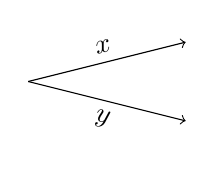
\begin{tikzpicture}
\draw[->] (0,0) -- (2,0.5) node[pos=.5,sloped,above] {$x$};
\draw[->] (0,0) -- (2,-.5) node[pos=.5,sloped,below] {$y$};
\end{tikzpicture} &
\begin{lstlisting} [language={[LaTeX]TeX},basicstyle=\ttfamily]
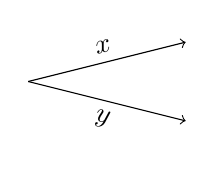
\begin{tikzpicture}
\draw[->] (0,0) -- (2,0.5) node[pos=.5,sloped,above] {$x$};
\draw[->] (0,0) -- (2,-.5) node[pos=.5,sloped,below] {$y$};
\end{tikzpicture}
\end{lstlisting}\\
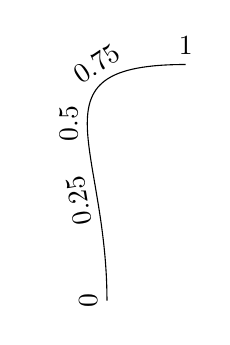
\begin{tikzpicture}
\tikzstyle{every node} = [sloped,above, %
allow upside down]
\draw (0,0).. controls +(up:2cm) and +(left:2cm) ..(1,3)
\foreach \p in {0,0.25,...,1} {node[pos=\p]{\p}};
\end{tikzpicture} &
\begin{lstlisting} [language={[LaTeX]TeX},basicstyle=\ttfamily]
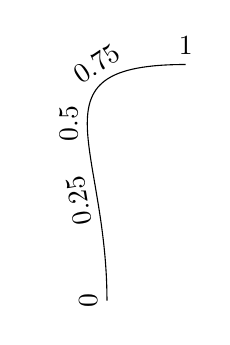
\begin{tikzpicture}
\tikzstyle{every node} = [sloped,above, %
allow upside down]
\draw (0,0).. controls +(up:2cm) and +(left:2cm) ..(1,3)
\foreach \p in {0,0.25,...,1} {node[pos=\p]{\p}};
\end{tikzpicture}
\end{lstlisting}
\end{tabular}
\item Simple computations are possible inside TikZ \\

\begin{tabular}{c|l}

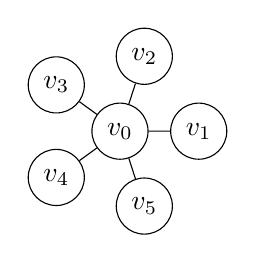
\begin{tikzpicture}
\tikzstyle{every node}=[draw,shape=circle];
\node (v0) at (0:0) {$v_0$};
\node (v1) at ( 0:1) {$v_1$};
\node (v2) at ( 72:1) {$v_2$};
\node (v3) at (2*72:1) {$v_3$};
\node (v4) at (3*72:1) {$v_4$};
\node (v5) at (4*72:1) {$v_5$};
\draw (v0) -- (v1)
(v0) -- (v2)
(v0) -- (v3)
(v0) -- (v4)
(v0) -- (v5);
\end{tikzpicture} &
\begin{lstlisting} [language={[LaTeX]TeX},basicstyle=\ttfamily]
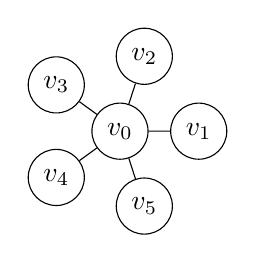
\begin{tikzpicture}
\tikzstyle{every node}=[draw,shape=circle];
\node (v0) at (0:0) {$v_0$};
\node (v1) at ( 0:1) {$v_1$};
\node (v2) at ( 72:1) {$v_2$};
\node (v3) at (2*72:1) {$v_3$};
\node (v4) at (3*72:1) {$v_4$};
\node (v5) at (4*72:1) {$v_5$};
\draw (v0) -- (v1)
(v0) -- (v2)
(v0) -- (v3)
(v0) -- (v4)
(v0) -- (v5);
\end{tikzpicture}
\end{lstlisting}\\
\hline
\begin{tikzpicture}
\coordinate [label=left:$A$] (A) at (0,0);
\coordinate [label=right:$B$] (B) at (1.25,0.25);
\draw (A) -- (B);
\node (D) [draw,circle through=(B),label=left:$D$] at (A) {};
\node (E) [draw,circle through=(A),label=right:$E$] at (B) {};
\coordinate[label=above:$C$] (C) at (intersection 1 of D and E);
\coordinate[label=above:$C'$] (Cp) at (intersection 2 of D and E);
\draw [red] (A) -- (C);
\draw [red] (B) -- (Cp);
\end{tikzpicture} &
\begin{lstlisting} [language={[LaTeX]TeX},basicstyle=\ttfamily]
\usetikzlibrary{calc,through}
\begin{tikzpicture}[scale=1.2]
\coordinate [label=left:$A$] (A) at (0,0);
\coordinate [label=right:$B$] (B) 
 at (1.25,0.25);
\draw (A) -- (B);
\node (D) 
 [draw,circle through=(B),label=left:$D$]
 at (A) {};
\node (E) 
 [draw,circle through=(A),label=right:$E$]
 at (B) {};
\coordinate[label=above:$C$] (C) 
 at (intersection 1 of D and E);
\coordinate[label=above:$C'$] (Cp) 
 at (intersection 2 of D and E);
\draw [red] (A) -- (C);
\draw [red] (B) -- (Cp);
\end{tikzpicture}
\end{lstlisting}
\end{tabular}
\end{itemize}
\end{note}
	
\begin{note}[Loops]:\\
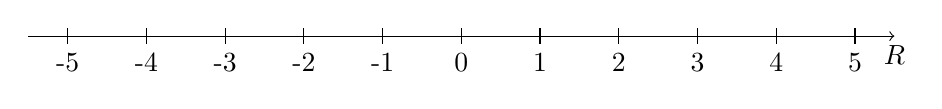
\begin{tikzpicture}
\draw[->] (-5.5,0) -- (5.5,0) node [below] {$\mathbb{R}$};
\foreach \x in {-5,...,5}
\draw (\x, 0.1) -- (\x, -0.1) node [below] {\x};
\end{tikzpicture}
\begin{lstlisting} [language={[LaTeX]TeX},basicstyle=\ttfamily]
\draw[->] (-5.5,0) -- (5.5,0) node [below] {$\mathbb{R}$};
\foreach \x in {-5,...,5}
\draw (\x, 0.1) -- (\x, -0.1) node [below] {\x};
\end{lstlisting}


\begin{tikzpicture}
\foreach \x in {1,3,...,10}
{
\shade[ball color=green!\x 0!red] (\x,0) circle (3mm);
}
\end{tikzpicture}
\begin{lstlisting} [language={[LaTeX]TeX},basicstyle=\ttfamily]
\foreach \x in {1,3,...,10}
{
\shade[ball color=green!\x 0!red] (\x,0) circle (3mm);
}
\end{lstlisting}
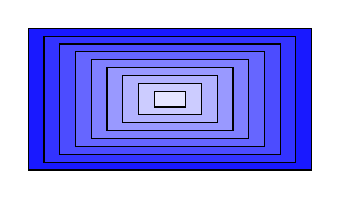
\begin{tikzpicture}
\foreach \x in {9,...,1}
\draw[fill=blue!\x0] (-0.2*\x , -0.1*\x )
rectangle (0.2*\x , 0.1*\x );
\end{tikzpicture}
\begin{lstlisting} [language={[LaTeX]TeX},basicstyle=\ttfamily]
\foreach \x in {9,...,1}
\draw[fill=blue!\x0] (-0.2*\x , -0.1*\x ) rectangle (0.2*\x , 0.1*\x );
\end{lstlisting}
\end{note}

\begin{note}[Some Samples]:\\
\begin{center}
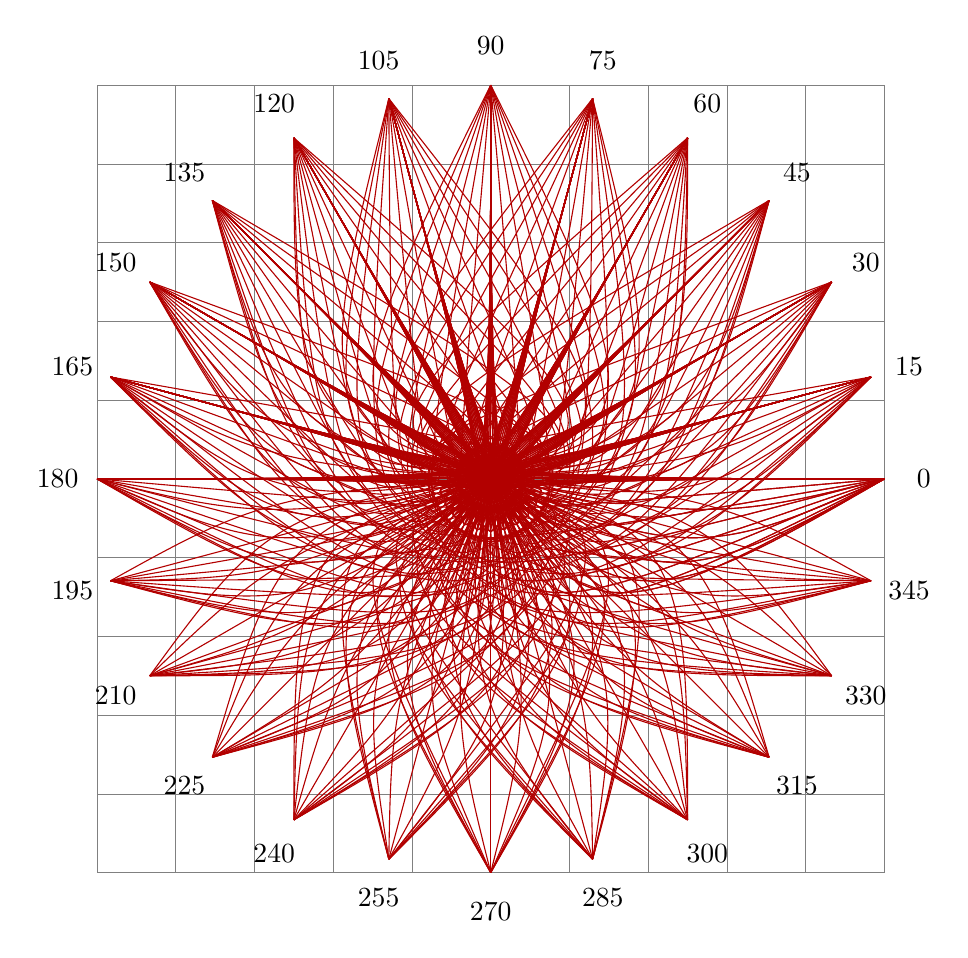
\begin{tikzpicture}
\draw[help lines] (-5,-5) grid (5,5);
\foreach \x in {0,15,...,350}
\node (n \x) at ( \x : 5.5) {\x};
\foreach \x in {0,15,...,180} 
\foreach \y in {0,15,...,360}
\draw[red!70!black] (\x:5) .. controls (\x:-2.5) .. (\y:5);
\end{tikzpicture}
\end{center}
\begin{lstlisting} [language={[LaTeX]TeX},basicstyle=\ttfamily]
\draw[help lines] (-5,-5) grid (5,5);
\foreach \x in {0,15,...,350}
\node (n \x) at ( \x : 5.5) {\x};
\foreach \x in {0,15,...,180} 
\foreach \y in {0,15,...,360}
\draw[red!70!black] (\x:5) .. controls (\x:-2.5) .. (\y:5);
\end{lstlisting}

\begin{center}

\begin{tikzpicture}[even odd rule]
\fill[clip] (0,0) circle (2cm) (60:2.5cm) arc (60:-60:2.5) (60:3cm) arc (60:-60:3cm);
\end{tikzpicture}

\begin{lstlisting} [language={[LaTeX]TeX},basicstyle=\ttfamily]

\begin{tikzpicture}[even odd rule]
\fill[clip] (0,0) circle (2cm) (60:2.5cm) 
arc (60:-60:2.5) (60:3cm) arc (60:-60:3cm);
\end{tikzpicture}
\end{lstlisting}
\end{center}

\begin{center}
	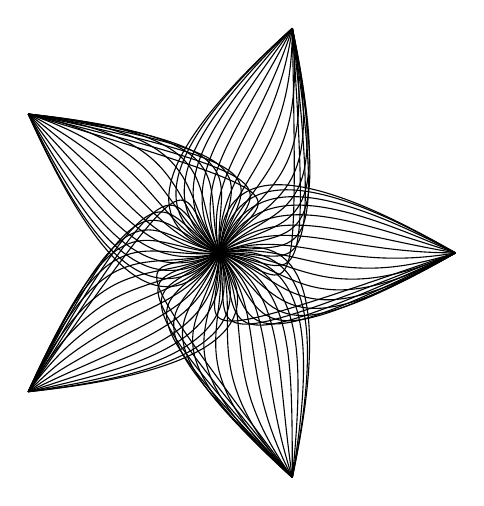
\begin{tikzpicture}
	\foreach \y in {0,360/5,2*360/5,3*360/5,4*360/5}
	\foreach \x in {-90,-80,...,90}
	\draw (0,0) .. controls (\x+\y:1) and (\x+\y-30:1.5) .. (\y:3);
	\end{tikzpicture}
	
	\begin{lstlisting} [language={[LaTeX]TeX},basicstyle=\ttfamily]
\foreach \y in {0,360/5,2*360/5,3*360/5,4*360/5}
\foreach \x in {-90,-80,...,90}
\draw (0,0) .. controls (\x+\y:1) and (\x+\y-30:1.5) .. (\y:3);
	\end{lstlisting}
\end{center}
\begin{center}
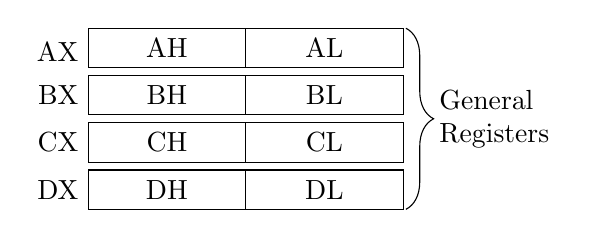
\begin{tikzpicture}
\node[left] at (0,0.25) {DX};
\draw (0,0) rectangle (2,.5) node [pos=0.5] {DH};
\draw (2,0) rectangle (4,.5) node [pos=0.5] {DL};

\node[left] at (0,0.85) {CX};
\draw (0,0.6) rectangle (2,1.1) node [pos=0.5] {CH};
\draw (2,0.6) rectangle (4,1.1) node [pos=0.5] {CL};

\node[left] at (0,1.45) {BX};
\draw (0,1.2) rectangle (2,1.7) node [pos=0.5] {BH};
\draw (2,1.2) rectangle (4,1.7) node [pos=0.5] {BL};

\node[left] at (0,2) {AX};
\draw (0,1.8) rectangle (2,2.3) node [pos=0.5] {AH};
\draw (2,1.8) rectangle (4,2.3) node [pos=0.5] {AL};

\draw [decorate,decoration={brace,amplitude=10pt,mirror},xshift=1pt,yshift=0pt]
(4,0) -- (4,2.3) node [black,midway,right,xshift=0.3cm,text width=1.5cm] 
{General Registers};
\end{tikzpicture}
\begin{lstlisting}[language={[LaTeX]TeX},basicstyle=\ttfamily]
\node[left] at (0,0.25) {DX};
\draw (0,0) rectangle (2,.5) node [pos=0.5] {DH};
\draw (2,0) rectangle (4,.5) node [pos=0.5] {DL};

\node[left] at (0,0.85) {CX};
\draw (0,0.6) rectangle (2,1.1) node [pos=0.5] {CH};
\draw (2,0.6) rectangle (4,1.1) node [pos=0.5] {CL};

\node[left] at (0,1.45) {BX};
\draw (0,1.2) rectangle (2,1.7) node [pos=0.5] {BH};
\draw (2,1.2) rectangle (4,1.7) node [pos=0.5] {BL};

\node[left] at (0,2) {AX};
\draw (0,1.8) rectangle (2,2.3) node [pos=0.5] {AH};
\draw (2,1.8) rectangle (4,2.3) node [pos=0.5] {AL};

\draw [decorate,decoration={brace,amplitude=10pt,mirror}
 ,xshift=1pt,yshift=0pt]
(4,0) -- (4,2.3) node [black,midway,right,xshift=0.3cm,text width=1.5cm] 
{General Registers};
\end{lstlisting}
\end{center}
\end{note}


\chapter{Linux: Tips and tricks}
\begin{note}[Export permanently]:\\
Add the export commands to the ~/.bashrc file.\\
\verb|export GOPATH=/home/hamidreza/workspace|\\
\verb|export PATH=$PATH:$GOROOT/bin:$GOPATH/bin|
\end{note}
\begin{note}[Using curl]:\\
Json Post request:\\
\verb|curl \|\\
\verb|	-X POST \|\\
\verb|	http://localhost:1323/users \|\\
\verb|	-H 'Content-Type: application/json' \|\\
\verb|	-d '{"name":"Joe","email":"joe@labstack"}'|\\\\
Post request:\\
\verb|curl \|\\
\verb|	-X POST \|\\
\verb|	http://localhost:1323/users \|\\
\verb|	-d 'name=Joe' \|\\
\verb|	-d 'email=joe@labstack.com'|\\\\
Get request: \\
\verb|curl \|
\verb|	-X GET \|
\verb|	http://localhost:1323/users\?name\=Joe\&email\=joe@labstack.com|
\end{note}
\chapter{Low Level Programming}
\section{Assembly Tips \& Tricks}
\section{C++ Tips \& Tricks}
\begin{note}[Visual C++ common headers]:\\
\begin{lstlisting} [language={c++}]
#include <cstdio>
#include <iostream> // for cout, cin, printf , ...
\end{lstlisting}
\end{note}

\begin{note}[\_\_Line\_\_ ] is a preprocessor command for line number in source code. look at note.\ref{ntInlineAsmMacro}
\end{note}

\begin{note}[Passing arrays to a function]
\begin{enumerate}
	\item Arrays can be very large so passing them as values is inefficient, therefore arrays always passed as an pointer.
	\item Arrays always passed to function as pointers, so they can be so their place (1st parameter, 2nd or else) does not matter.
\end{enumerate}
\begin{lstlisting} [language={c++}]
int main (void) 
{
   double values[] = {1.0, 2.0, 3.0, 4.5};
   cout << average (values, (sizeof values)/(sizeof values[0]))
}
double average (double array[], int count) {...}
\end{lstlisting}
\end{note}

\begin{note}[CallByRef (\&) and CallByPointer (*)]
\begin{lstlisting}[language={c++}]
void inc10p (int* n) { *n += 10;}
void inc10r (int& n) { n += 10;}
void inc10v (int n) { n += 10;}
int main(int argc, char *argv[])
{
   int n = 10;
   inc10p(&n); cout << n << endl; //prints 20
   inc10r(n);  cout << n << endl; //prints 30
   inc10v(n);  cout << n << endl; //prints 30
   return 0;
}
\end{lstlisting}
\end{note}

\begin{note}[``const'' after a function]

``const'' after a function declaration means that the function is not allowed to change any class members (except ones that are marked mutable). for example
\begin{lstlisting} [language={c++}]
class Foo {
public:
   int Bar(int Random_Argument) const
   {
      _tmp = 3; //Class member changed -- error
      return Random_Argument * 2;
   }
private:
   int _tmp;
};
\end{lstlisting}
The program wont compile cause Function Bar is defined constant but the value of \_tmp (which is a class member) has changed in it.\\

Consider two class-typed variables:
\begin{lstlisting} [language={c++}]
class Boo { ... };

Boo b0;       // mutable object
const Boo b1; // non-mutable object
\end{lstlisting}
Now you are able to call any member function of Boo on b0, but only const-qualified member functions on b1.
\end{note}

\subsection{lvalues, rvalues, move semantics and operator overriding}
Every C++ expression is either an lvalue (left or locater value) or an rvalue (right value). An lvalue refers to an object that persists beyond a single expression. You can think of an lvalue as an object that has a name. All variables, including non-modifiable (const) variables, are lvalues. An rvalue is a temporary value that does not persist beyond the expression that uses it. 
\begin{note}[Some examples of lvaues and rvalues]
\begin{lstlisting}
//Incorrect usage:
//   - y is a reference, can not be assigned to a temporary value
int& y = 10; 
//Correct usage:
int x = 10;
int& y = x;

// Correct usage: the conditional operator returns an lvalue.
((i < 3) ? i : j) = 7;
\end{lstlisting}
\end{note}
\begin{note}[Lvalues - Returning a reference]
\begin{enumerate}
\item Have u seen a function used in the left side of an assignment before? :D
\item You can also return an lvalue reference from a function. like: \\ \lstinline[columns=fixed]{double& lowest(double a[], const int& len)} - notice to double\&
\item References as return types are of primary significance in the context of object-oriented programming. they enable you to do things that would be
impossible without them. (This particularly applies to “operator overloading”)
\end{enumerate}
\begin{lstlisting} [language={c++}]
double& lowest(double values[], const int& length); // Function prototype
int main(void)
{
   double data[] = { 3.0, 10.0, 1.5, 15.0, 2.7, 23.0,
	4.5, 12.0, 6.8, 13.5, 2.1, 14.0 };
   int len(_countof(data)); // Number of elements

   lowest(data, len) = 6.9; // Change lowest to 6.9
   lowest(data, len) = 7.9; // Change lowest to 7.9
}
// Function returning a reference
double& lowest(double a[], const int& len)
{
   int j(0); // Index of lowest element
   for(int i = 1; i < len; i++)
      if(a[j] > a[i]) // Test for a lower value...
         j = i; // ...if so update j
   return a[j]; // Return reference to lowest element
   /*Remember that arrays are ALWAYS passed to functions as an pointers
   So a[] is actuall a pointer to data[], this is
   why that the function return value
   changes the value of the lowest member of the data array.*/
}
\end{lstlisting}
\end{note}

\begin{note}[Rvalue - Returning a rvalue reference can cause a catastrophe]
\begin{lstlisting} [language={c++}]
Beta_ab&&
Beta::toAB() const {
return move(Beta_ab(1, 1));
}
\end{lstlisting}
This returns a dangling reference, just like with the lvalue reference case. After the function returns, the temporary object will get destructed. You should return Beta\_ab by value, like the following:
\begin{lstlisting} [language={c++}]
Beta_ab
Beta::toAB() const {
return Beta_ab(1, 1);
}
\end{lstlisting}
Now, it's properly moving a temporary Beta\_ab object into the return value of the function. If the compiler can, it will avoid the move altogether, by using RVO (return value optimization).
\end{note}

\begin{note}[An in depth complete example]

In this example, we build the Intvec class which is a dynamically sized vector of integers. We also implement + and = operators.
\begin{lstlisting} [language={c++}]
class Intvec
{
public:
   explicit Intvec (size_t num = 0)
      : m_size(num), m_data(new int[m_size])
   {
      for (uint i=0; i < m_size ; i++ ) m_data[i] = 1;
      log("constructor");
   }

   ~Intvec ()
   {
      log("destructor");
      if (m_data) {
         delete[] m_data;
         m_data = 0;
      }
   }
   
   void exposure ()
   {
      qDebug() << "[" << this << "] m_size: " << m_size;
      std::cout << "[ " << this << " ] m_data: ";
      for (uint i=0; i < m_size ; i++ )
         std::cout << m_data[i];  std::cout << endl;
   }
private:
   size_t m_size;
   int* m_data;
   void log(const char* msg)
   {
      qDebug() << "[" << this << "] " << msg;
   }
};
\end{lstlisting}
\textbf{Phase 1: Adding a default copy constructor.}\\
Constructing an instance of this class from another instance, requires a default copy constructor. for example:
\begin{lstlisting} [language={c++}]
Intvec v1(10);
Intvec v2(v1); // this instance is copy of v1, needs default constructor
\end{lstlisting}
\begin{remark} \label{rmkDefaultCopyConstructor}
	C++ compiler provides default copy constructor same as assignment operator. The default version simply provide a member-by-member copying process, similar to that of the default copy constructor. But it's crucial to remember that for any class that has
	space for members allocated dynamically, you must implement the assignment operator (same as copy constructor) manually.
\end{remark}
The memory needed for m\_data in our class is allocated dynamically, so we cannot use default copy constructor (according to remark.\ref{rmkDefaultCopyConstructor}), But what happens if we use it? disaster will result! Since each object will have a pointer to the same
m\_data, if it is changed for one object, it’s changed for both. There is also the problem that when one object is destroyed, its destructor will free the memory used for the m\_data, and the other object will be left with a pointer to memory that may now be used for something else.
\begin{lstlisting} [language={c++}]
Intvec (const Intvec& v)
   //Using by reference parameter simply saves the amout of memory needed.
   : m_size(v.m_size) , m_data(new int[v.m_size])
   //explicit defination of m_data and m_size 
{
   for (uint i=0; i < m_size ; i++ ) m_data[i] = v.m_data[i];
   log("overrided copy constructor");
}
// now without any problem  we have Intvec v2(v1);
\end{lstlisting}
\textbf{Phase 2: Adding assignment operator.}\\
Like copy constructor, we need to override assignment operator with an appropriate (according to remark.\ref{rmkDefaultCopyConstructor}) before being able to use instructions like v2=v1;
\begin{lstlisting} [language={c++}]
Intvec& operator=(Intvec& other)
{
   log("copy assignment constructor");
   delete[] m_data; //relese memory for lhs operand
   m_size = other.m_size;
   m_data = new int[m_size];
   for (uint i=0; i < m_size ; i++ )
      m_data[i] = other.m_data[i];
   return *this;
}
\end{lstlisting}
An assignment might seem very simple, but there’s a couple of subtleties that need further
investigation. First of all, note that you return a reference from the assignment operator function. It may not be immediately apparent why this is so — after all, the function does complete the assignment operation entirely, and the object on the right of the assignment will be copied to that on the left. Superficially, this would suggest that you don’t need to return anything, but you need to consider in a little more depth how the operator might be used.
\begin{remark}
	When implementing assignment operator, we often return a reference to an object instead of object itself.
\end{remark}
If the Intvec object itself had been returned instead of a reference to it, insteructions like \verb|(v3 = v2) = v1;| wouldn't have worked correct. This legitimate instruction translates into \verb|(v3.operator=(v2)).operator=(v1);|. In this situation, object returned by \verb|operator=()| is used to call the \verb|operator=()| which is illigal because it's a temporary rvalue. hence the return value should be a reference\\ \\
\textbf{Phase 3: Adding addition operator.}
\begin{lstlisting} [language={c++}]
//returning Intvec& or Intvec&& will result in a dangling reference
//cause temporary objects are destroyed at the end of function.
//we also pass rhs by ref cause it's more efficent and takes less memory
Intvec operator+(const Intvec& rhs)
{
   //we want lhs object untouched, so we make a copy of it
   Intvec tmp(*this);
   for (uint i=0; i<tmp.m_size; i++)
      tmp.m_data[i] += rhs.m_data[i];
   return tmp;
}
\end{lstlisting}
Right now statements like \verb|v2 + v1;| works perfectly but what about \verb|v3 = v2 + v1;|? If we try it, the compiler will complain of \textit{``invalid initialization of non-const reference of type `Intvec\&' from an rvalue of type `Intvec'.''}It's brought about the fact that our assignment operator work by ref (which only accepts lvalues).\\ \\
\textbf{Phase 4: Handling the problem: Fixing assignment operator}\\
Here we have two choices, either changing \verb|Intvec& operator=(Intvec& other)| to \verb|Intvec& operator=(Intvec other)| which works faultlessly well, or add another assignment operator which comes below:
\begin{lstlisting} [language={c++}]
Intvec& operator=(Intvec&& other)
{
   log("copy assignment constructor");
   delete[] m_data; //relese memory for lhs operand
   m_size = other.m_size;
   m_data = new int[m_size];
   for (uint i=0; i < m_size ; i++ )
      m_data[i] = other.m_data[i];
   return *this;
}
\end{lstlisting}

\end{note}

\subsection{Templates}
Templates are a feature of the C++ programming language that allows functions and classes to operate with generic types. This allows a function or class to work on many different data types without being rewritten for each one.
\begin{note}[Template Functions and Class]\\
Function Templates are defined like:
\begin{lstlisting} [language={c++}]
template <class identifier> function_declaration;
template <typename identifier> function_declaration;
\end{lstlisting}
For example Function Max will return maximum of two given values in different types.
\begin{lstlisting} [language={c++}]
template <typename Type>
Type max(Type a, Type b) {
   return a > b ? a : b;
}
\end{lstlisting}
The basic syntax for declaring a templated class is as follows:
\begin{lstlisting} [language={c++}]
template <class a_type> class a_class {...};
\end{lstlisting}
An example of usage are presented below. In this example, multiply function is implemented outside of the class using template functions.
\begin{lstlisting} [language={c++}]
template <class A_Type> class calc
{
public:
   A_Type multiply(A_Type x, A_Type y);
   A_Type add(A_Type x, A_Type y)
   {
      return x+y;
   }
};
template <class A_Type> A_Type calc<A_Type>::multiply(A_Type x,A_Type y)
{
   return x*y;
}
// down there in main
calc<int> c;
cout << c.add(2,3);
\end{lstlisting}
\end{note}

\begin{note}[Virtual Functions and Abstract Classes (Interfaces)]

An interface describes the behavior or capabilities of a C++ class without committing to a particular implementation of that class. A class is made abstract by declaring at least one of its functions as pure virtual function. A pure virtual function is specified by placing "= 0" in its declaration as follows:
\begin{lstlisting} [language={c++}]
template <typename t> class Box
{
public:
   // pure virtual function
   virtual t getVolume() const = 0;
protected:
   t length;      // Length of a box
   t breadth;     // Breadth of a box
   t height;      // Height of a box
};
\end{lstlisting}
So each box need have been provided by getVolume method.
\begin{lstlisting} [language={c++}]
template <typename t> class NormalBox : public Box<t>
{
public:
   NormalBox (t _x,t _y ,t _z)
   {
      this->length = _x; this->breadth = _y; this->height = _z;
   }

   double getVolume() const
   {
      return this->length * this->breadth * this->height;
   }
};

template <typename t> class CubicBox : public Box<t>
{
public:
   CubicBox (t _x);
   t getVolume() const
   {
      return this->length * this->length * this->length;
   }
};
//Constructor Definition
template <typename t> CubicBox<t> :: CubicBox (t _x) 
{
   this->length = this->breadth = this->height = _x;
}
\end{lstlisting}
\end{note}

\section{Embedded assembly in C++}
\begin{note}[Embedding a byte in Code Area]

\begin{lstlisting}[language={c++}]
__asm{
  some code
  jmp after
  _emit 0x0f
		
after:
  mov eax,eax
}
\end{lstlisting}
\end{note}

\begin{note}[C++ Inline assembly in macros]\label{ntInlineAsmMacro}

Sometimes we want to insert some junk codes, between each line of the program, the best solution is to write a macro to simplify the process instead of inserting the same redundant ASM code frequently. e.g.:

\begin{lstlisting}[language={c++}]
#define Paste (a,b) a##b
#define PasteSymbols (a,b) Paste (a,b)
\end{lstlisting}
\_\_Line\_\_ wont work properly without two above definitions. So they are required.

\begin{remark}
Notice that labels usually should be unique in inline assembly to prevent unwanted jumps and incorrect breakdown in control flow. therefore labels have to be defined like below:
\begin{lstlisting}[language={c++}]
_asm {PasteSymbols (Label,__LINE__): }
\end{lstlisting}
\end{remark}
Final macro looks like:
\begin{lstlisting}[language={c++}]
#define IncDecJmpBetween () \
	_asm {inc eax};\
	_asm {jmp PasteSymbols (Label,__LINE__)};\
	_asm {PasteSymbols (Label,__LINE__):};\
	_asm {dec eax};
\end{lstlisting}
\end{note}

\section{C++ Standard Library}
\begin{note}[Pair]
\begin{lstlisting}[language={c++}]
#include <map>
#include <string>
int main(){
  std::pair<int,std::string> one (1,"One");
  std::pair<int,std::string> two_and_three[] = { {2,"Two"} , {3,"Three"} };
  std:cout << "1 is " << one.second << " and 2 is " << two_and_three[0].second;
}
\end{lstlisting}
\end{note}
\begin{note}[Vector and Iterators]
\begin{itemize}
\item vector definition:
\begin{lstlisting}[language={c++}]
std::vector<std::string> v = {"This","is"}
\end{lstlisting}
\item push and pop:
\begin{lstlisting}[language={c++}]
v.push_back("an");
v.pop_back();
\end{lstlisting}
\item remove an item:
\begin{lstlisting}[language={c++}]
v.erase(v.begin() + 4); //removes the 4th item
v.erase(std::remove(v.begin(),v.end(),"is"));
//This one uses std::remove to remove a time by it's value instead of 
//it's position. It's called erase-remove idiom.
\end{lstlisting}
\item Iterator:
\begin{lstlisting}[language={c++}]
std::vector<std::string>::iterator it;
for (it = v.begin(); it < v.end(); it++)
  std::cout << *it << std::endl;
\end{lstlisting}
\item using auto:
\begin{lstlisting}[language={c++}]
for (auto it = v.begin(); it < v.end(); it++)
  std::cout << *it << std::endl;
\end{lstlisting}
\item using foreach:
\begin{lstlisting}[language={c++}]
foreach (auto str : v)
//In Qt, foreach (auto str, v)
	std::cout << v << std::endl;
\end{lstlisting}
\end{itemize}
\end{note}
\chapter{Python}

\begin{note}[Strings, Bytes, Lists, Dictionaries]
\begin{lstlisting}[language = {python}]
#Strings
s = "you" "can" "concat" "strings"
s = "he"+'l'*2+'o'
s = "this is a String\n"
multiline_string = """this is 
                      a multiline 
                      string"""
raw_string = r'c:\windows\blah\blah\blah'

s.capitalize() # "This is a string"
s.split() # ['this', 'is', 'a', 'string']
s.find('a') # 8

if 'this' in s:
   print ("true")
   
s.count('is') # 2 - number of non-verlaping substrings
s[5]   # 'i'
s[5:]  # 'is a string'
s[5:7] # 'is'
s[-3:] # 'ing'

#Bytes
b = b"i'm a byte stream"

#Lists
l = []
l = [1 , 2, 'a' , "aaa"]
l.append (4.145)
list("characters") # ['c', 'h', 'a', 'r', 'a', 'c', 't', 'e', 'r', 's']

#Dictionaries
d = {}
d = {'alice':'001-4234-234', 'bob':'002-2341-455'}
d['charls'] = '001-8797-009' #inserts into dictionary
\end{lstlisting}
\end{note}
\begin{note}[Modularity]\\
	Modules are .py files, while packages are folders containing modules and other packages.
	\\
	\\
In math2.py:
\begin{lstlisting}[language = {python}]
class basic_math:
   def power_two(a):
      return a*a
\end{lstlisting}
In main.py:
\begin{lstlisting}[language = {python}]
from math.py import basic_math

print("the power two of 2 is ", basic_math.power_two(2))
\end{lstlisting}
\end{note}
\begin{note}[Distinguishing between module import and module executions]
\begin{lstlisting}[language = {python}]
#in math.py
print(__name__)
# when imported prints math
# when executed like python3 math.py
# prints __main__

import sys

if (__name__ = "__main__"):
   main(sys.argv[1]) #when executed, run main with first command line argument
\end{lstlisting}
\end{note}

\begin{note}[Docstrings]
\begin{lstlisting}[language = {python}]
def Power_Two(n):
    """ Computes the square of a given number
    
    Args:
        n: the number we want to compute it's square
        
    Returns:
        square of given number
    """
    return n*n
\end{lstlisting}
now we can see the document using help(Power\_Two)
\end{note}
\begin{note}[Python has dynamic and strong type system]
\begin{lstlisting}[language = {python}]
def add(a, b):
    return a + b
#these are all acceptable (because of dynamic)
add(1,2)
add("qwe", "rty")
add(['asd','aaa'],["zxc","wqe"])
add(1.2,2.3)
#but this is not (because of strong)
add("string", 42)
\end{lstlisting}
\end{note}
\begin{note}[Scope]
\begin{lstlisting}[language = {python}]
count = 0
def show_count():
    print("the count is " , count) #works, cause there is no local count
    
def set_count(c)
    count = c # creates a local var count, and sets it
    global count = c # sets the value of the global count
\end{lstlisting}
\end{note}
\begin{note}[Tuples]
\begin{enumerate}
	\item Tuples are defined with parenthesis() instead of brackets[]
	\item Tuples are like lists, but with special usages.
	\item One of the tuple usages are return value of the functions
\end{enumerate}
\begin{lstlisting}[language = {python}]
def minmax(l):
    return min(l), max(l)

l = [1,23,43,12,43,55,6,34,9]
minmax(l) # (1, 55)
lower, upper = minmax(l)

#another usage
(a,(b,c)) = (1,(2,3))
# now a = 1, b = 2 and c = 3

if 1 in (1,2,3,4):
    print ("True")
\end{lstlisting}
\end{note}
\begin{note}[Strings, in more details]
\begin{lstlisting}[language = {python}]
len("hamid") # 5

#Join
s = " ".join(['this','is','a','string'])

#partition
departure, seperator, arrival = "London:Edinburgh".partition(':')
departure # 'London'

#format
"My name is {} and i'm {}".format("hamid",22)

import math
"Math constants: pi={m.pi}, e={m.e}".format(m=math)
# 'Math constants: pi=3.141592653589793, e=2.718281828459045'
\end{lstlisting}
\end{note}
\begin{note}[Range]
\begin{lstlisting}[language = {python}]
list(range(5)) # [0, 1, 2, 3, 4]
l=list(range(10,20,2))
for i in l:
    print(i,end=' ');
# 10 12 14 16 18 

for i, v in enumerate(l):
    "The index is {} and the value is {}".format(i,v)
    
# 'The index is 0 and the value is 10'
# 'The index is 1 and the value is 12'
# 'The index is 2 and the value is 14'
# 'The index is 3 and the value is 16'
# 'The index is 4 and the value is 18'
\end{lstlisting}
\end{note}

\begin{note}[Exceptions]\\
	Different types of exceptions in python are: IndexError, ValueError, TypeError, KeyError, OSError and etc.
\begin{lstlisting}[language = {python}]
def convert(s):
'''Convert to an integer.'''
   try:
      x = int(s)
      print("Conversion succeeded")
      return x
   except (ValueError, TypeError, OSError) as e:
      print("conversion error: {}".format(str(e)))
   finally:	
      print("End of Function")
\end{lstlisting}

\end{note}
\begin{note}[Comprehensions]\\
The general form of list comprehensions is: [expr(item) for item in iterable]
\begin{lstlisting}[language = {python}]
words = "This is a total useless text".split()
[len(word) for word in words]
>>> [4, 2, 1, 5, 7, 4]
from math import factorial
[(x,factorial(x)) for x in range(10)]
>>> [(0, 1), (1, 1), (2, 2), (3, 6), (4, 24), (5, 120), (6, 720),
     (7, 5040), (8, 40320), (9, 362880)
    ]
\end{lstlisting}
The general form of set comprehensions is: \{expr(item) for item in iterable\}.\\
It's possible to filter comprehensions using if:
\begin{lstlisting}[language = {python}]
def is_prime(x):
   ...
   
#list all the prime numbers less than 100
[x for x in range(100) if is_prime(x)]

#get list of all digits in a number: for examle [1, 2, 3] for 123
digits = [int(x) for x in list(str(x))]
\end{lstlisting}
\end{note}
\chapter{QT}
\section{Basics}
\begin{note}[QDebug header]\\
\verb|#include <QDebug>| and usage like \verb|qDebug() << "[" << this << "] m_size: " << m_size;|
\end{note}

\begin{note}[Signals and Slots]
\begin{enumerate}
\item In form designer, there is a signal/slot view (F4) which assist to define new signal/slots.
\item To add or remove s/s manually we can use \verb|connect| and \verb|disconnect|
\end{enumerate}
\begin{lstlisting} [language={c++}]
MainWindow::MainWindow(QWidget *parent) :
QMainWindow(parent), ui(new Ui::MainWindow)
{
  ui->setupUi(this);

  connect(ui->horizontalSlider,SIGNAL(valueChanged(int))
            ,ui->progressBar,SLOT(setValue(int)));
}
\end{lstlisting}
\end{note}

\begin{note}[Actions]
	
When you create a new menu, an action will be created, which can be drag and dropped on the toolbar. an actions allows u to trigger an event. rightclick $\rightarrow$ go to slots.
\end{note}

\begin{note}[setCentralWidget(object o)]
	
	You can use this function to set an object as the main widget on the form.
\end{note}

\begin{note}[Dialogs]
\begin{enumerate}
\item After creating a dialog, you need to include it the mainwindow.cpp (the parent window.) \verb|#include "mydialog.h"|
\item To show the dialog:
\verb|Dialog myDialog; myDialog->setModal(true); myDialog->exec();|
\item if u use exec, u cannot show the dialog modaless. we need to use show method for modaless dialogs, and also we should not define the dialog in stack, we need to define it on heap, so after the show function, the respected object wont be destroyed.
\begin{lstlisting} [language={c++}]
//In mainwindow.h
#include <dialog.h>
...
class MainWindow : public QMainWindow
{
   ...
private:
   Dialog *myDialog = nullptr;
};
//In mainwindow.cpp
void MainWindow::on_actionNew_Dialog_triggered()
{
   myDialog = new Dialog(this); //set this form as the parent
   myDialog->setModal(false);
   myDialog->show();
}
\end{lstlisting}
\end{enumerate}
\end{note}

\begin{note}[Minimal application with HTML aware widgets]
\begin{lstlisting}[language = {c++}]
#include <QApplication>
#include <QLabel>
int main(int argc, char *argv[])
{
   QApplication a(argc, argv);
   QLabel *l = new QLabel("<b>Hello</b> <font color=red><i>world");
   l->show();
   return a.exec();
}
\end{lstlisting}
\end{note}

\begin{note}[QHBoxLayout and QVBoxLayout]
\begin{enumerate}
	\item QHBoxLayout and QVBoxLayout are not widgets, so u cant show them unless u make a widget.
	\item There is a example below.
\end{enumerate}
\begin{lstlisting}[language = {c++}]
#include <QApplication>
#include <QLabel>
#include <QPushButton>
#include <QHBoxLayout>

int main(int argc, char *argv[])
{
  QApplication a(argc, argv);
  QLabel *l = new QLabel("<b>Hello</b> <font color=red><i>world");

  QWidget* window = new QWidget();
  QHBoxLayout* hlayout = new QHBoxLayout();

  hlayout->addWidget(new QPushButton("Hehe"));
  hlayout->addWidget(new QPushButton("HoHo"));
  hlayout->addWidget(new QPushButton("HerHer"));
  hlayout->addWidget(l);

  window->setLayout(hlayout);
  window->show();
  return a.exec();
}
\end{lstlisting}
\begin{center}
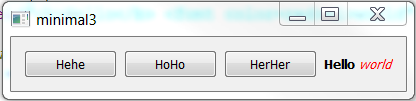
\includegraphics[]{Images/QT/HBox}
\end{center}
\end{note}

\begin{note}[QGridLayout]\\
Parameters in Order:\\
1.QWidget 2.Row Number 3.Column Number 4.Row Span 5.Column Span
\begin{lstlisting}[language = {c++}]
QGridLayout* main_layout = new QGridLayout(window);
main_layout->addWidget(new QPushButton("heheheh"),1,1,1,1);
main_layout->addWidget(new QPushButton("heheheh"),1,2,1,1);
main_layout->addWidget(new QPushButton("heheheh"),2,1,1,2);
\end{lstlisting}
\begin{center}
	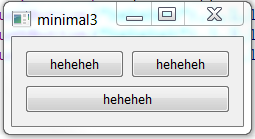
\includegraphics[]{Images/QT/QGrid}
\end{center}
\end{note}

\begin{note}[QSplitter]: u can add them by selection widgets in design view and click on the vertical/horizontal splitters
\end{note}

\begin{note}[QStatusBar]
\begin{lstlisting}[language = {c++}]
QLabel* lblStatusBar = new QLabel("Hi There");
...
ui->statusBar->addPermanentWidget(lblStatusBar);
ui->statusBar->showMessage("Hello",2000);
\end{lstlisting}
\end{note}

\begin{note}[QMessageBox]
\begin{lstlisting}[language = {c++}]
QString str[] = {"Hello","There"};
QMessageBox::critical(this,str[0],str[1],QMessageBox::YesAll);
\end{lstlisting}
\end{note}

\begin{note}[QTimer]
\begin{lstlisting}[language = {c++}]
QTimer* tmr = nullptr;

void main {
  tmr=new QTimer(this);
  tmr->setInterval(20);
  connect (tmr,SIGNAL(timeout()),this,SLOT(timerhit()));
  tmr->start();
}
//timerhit slot
void MainWindow::timerhit()
{
  ...
}
\end{lstlisting}
\end{note}

\begin{note}[Threads]
	
To build a thread, first we need to create a class that inherits from QThread and Q\_OBJECT should be emplaced in it.
\begin{lstlisting}[language = {c++}]
class Counter : public QThread
{
  Q_OBJECT
public:
  Counter();
};
\end{lstlisting}
Then we need to override the run() function. This is the thread entry. and also to provide bidirectional communication with the main thread, we need to define a signal, so it could be caught by the main thread if it was needed.
\begin{lstlisting}[language = {c++}]
class Counter : public QThread
{
  Q_OBJECT
private:
  bool blnStop = false;
public:
  Counter();
  void run() override;
signals:
  void NumberChanged (int);
};
void Counter::run() {
  static int i = 0;
  blnStop = false;
  while(!blnStop){
    //emit is used to raise the signal
    //it's equal to raise event in C#
    emit NumberChanged(++i);
    this->msleep(1);
  }
}
\end{lstlisting}
To find a way for stopping the thread from the outside, we can define a onQuit slot (or any other public function).
\begin{lstlisting}[language = {c++}]
public slots:
  void onQuit();
\end{lstlisting}
And finally to initialize and start it:
\begin{lstlisting}[language = {c++}]
void main ()
{
  c = new Counter();
  connect(c,SIGNAL(NumberChanged(int)),this,SLOT(onNumberChange(int)));
  c->start();
}
void MainWindow::onNumberChange(int i)
{
  ui->lblCount->setText(QString::number(i));
}
\end{lstlisting}
\end{note}
\begin{note}[QString]
\begin{itemize}
\item For converting numbers to QString
\begin{lstlisting}[language = {c++}]
Qstring str = QString::number(1);
\end{lstlisting}
\item For converting std::string to QString
\begin{lstlisting}[language = {c++}]
QString str = QString::fromStdString("AnSTDString");
\end{lstlisting}
\item For const char* to QString
\begin{lstlisting}[language = {c++}]
const char* psStr = "This is a string";
QString str(psStr);
\end{lstlisting}
\end{itemize}
\end{note}

\begin{note}[QList]
\begin{itemize}
\item It's like vector in std library;
\item Useful methods: append, removeat, removeOne, first, last, [], <<
\item it can be used in foreach loops
\end{itemize}
\begin{lstlisting}[language = {c++}]
QList<std::string> list = {"I","said"};
list.append("hello");
list.append("there");
list << "to" << "you";
list.removeOne("hello");
QString str(QString::fromStdString(list[0]));
\end{lstlisting}
\end{note}

\begin{note}[QListIterator]
\begin{enumerate}
	\item It's used for iteration trough lists.
	\item Useful methods: hasNext, hasPrevious, next, previous
	\item Use peekNext to preview next item.
\end{enumerate}
\begin{lstlisting}[language = {c++}]
QList<std::string> list = {"Hello","there","asdasd","qwerty"};
QListIterator<std::string> Iterator (list);
//next line is also valid
//QListIterator<std::string> Iterator = list;
while (Iterator.hasNext())
  qDebug() << QString::fromStdString(Iterator.next());
\end{lstlisting}
\end{note}

\begin{note}[QMap and QMapIterator]
\begin{enumerate}
\item It's used to map values to keys
\begin{lstlisting}[language = {c++}]
//QMap<key,value>
QMap<int,QString> employees = {{3,"Bob"},{2,"Hamid"}};
\end{lstlisting}
\item Useful methods: insert, value, key
\begin{lstlisting}[language = {c++}]
QMap<int,QString> employees = {{3,"Bob"},{2,"Hamid"}};

foreach (auto e, employees)
  qDebug() << e;

QMapIterator<int,QString> Iter (employees);
while (Iter.hasNext())
{
  Iter.next();
  qDebug() << Iter.key() << Iter.value();
}
\end{lstlisting}
\end{enumerate}
\end{note}
\begin{note}[QHash ]is equal to QMap in usage.
\end{note}
\begin{note}[QStringList]
\begin{lstlisting}[language = {c++}]
QStringList ls = QString("This is a test").split(' ');
foreach (auto s, ls)
  qDebug() << s;
ls.replaceInStrings("s","sos");
qDebug() << ls.join(",");
\end{lstlisting}
\end{note}

\begin{note}[QSort]
\begin{lstlisting}[language = {c++}]
QList<int> l = {3,2,4,1,0};
qSort(l);
foreach (int i, l) qDebug() << i;
\end{lstlisting}
\end{note}
\section{Windows Programming}
\begin{note}[Windows data types and naming]:\\
Here are a few of the most common windows types you are likely to meet:\\
\begin{center}
\begin{tabular}{|M{3cm}|M{12cm}|N}
\MyTabHeadings Type & \textbf{\textcolor{white}{Explanation}} &\\[\rowheight] \hline
\textbf{BOOL(BOOLEAN)} & A Boolean variable can have the values TRUE or FALSE. Note that this is not the same as the C++ type bool, which can have the values true or false. &\\ [\rowheight] \hline
\textbf{BYTE} & An 8-bit byte. &\\ [\rowheight] \hline
\textbf{CHAR} & An 8-bit character. &\\ [\rowheight] \hline
\textbf{DWORD} & A 32-bit unsigned integer that corresponds to type unsigned long in C++. &\\ [\rowheight] \hline
\textbf{HANDLE} & A handle to an object — a handle being a 32-bit integer value that records the location of an object in memory, or 64-bit when compiling for 64-bit. &\\ [\rowheight] \hline
\textbf{HBRUSH} & A handle to a brush, a brush being used to fi ll an area with color. &\\ [\rowheight] \hline
\textbf{HCURSOR} & A handle to a cursor. &\\ [\rowheight] \hline
\textbf{HDC} & Handle to a device context — a device context being an object that enables you to draw on a window. &\\ [\rowheight] \hline
\textbf{HINSTANCE} & Handle to an instance. &\\ [\rowheight] \hline
\textbf{LPARAM} & A message parameter. &\\ [\rowheight] \hline
\textbf{LPCTSTR} & LPCWSTR if \_UNICODE is defined, otherwise LPCSTR. &\\ [\rowheight] \hline
\textbf{LPCWSTR} & A pointer to a constant null-terminated string of 16-bit characters. &\\ [\rowheight] \hline
\textbf{LPCSTR} & A pointer to a constant null-terminated string of 8-bit characters. &\\ [\rowheight] \hline
\textbf{LPHANDLE} & A pointer to a handle. &\\ [\rowheight] \hline
\textbf{LRESULT} & A signed value that results from processing a message. &\\ [\rowheight] \hline
\textbf{WORD} & A 16-bit unsigned integer, so it corresponds to type unsigned short in
C++. &\\ [\rowheight] \hline
\end{tabular}
\end{center}

\newpage
A sample of the prefixes you might come across in \textit{Hungarian notation} is:\\
\begin{table}[h]
	\makegapedcells
	\centering
	\resizebox{\textwidth}{!}{%resizing the whole table
\begin{tabular}{|c|P{13cm}|}\hline
\textbf{PREFIX} & \textbf{MEANING} \\  \hline
\textbf{b} & a logical variable of type BOOL, equivalent to int \\   \hline
\textbf{by} & type unsigned char; a byte \\   \hline
\textbf{c} & type char \\   \hline
\textbf{dw} & type DWORD, which is unsigned long \\   \hline
\textbf{fn} & a function \\   \hline
\textbf{h} & a handle, used to reference something \\   \hline
\textbf{i} & type int \\   \hline
\textbf{l} & type long \\   \hline
\textbf{lp} & long pointer \\   \hline
\textbf{n} & type unsigned int \\   \hline
\textbf{p} & a pointer \\   \hline
\textbf{s} & a string \\   \hline
\textbf{sz} & a zero terminated string \\   \hline
\textbf{w} & type WORD, which is unsigned short \\   \hline
\end{tabular}
}
\caption{Hungarian notation sample prefix}
\end{table}

\end{note}
% !TeX spellcheck = <none>
\chapter{Go}
\section{Golang Fundamentals}
\begin{note}[Setup]:
	\begin{enumerate}
		\item To install go use:\\
		\verb|sudo apt install go|
		\item
		Create a new directory for GO\_PATH and add \\
		\verb|export GOPATH=GO_PATH|\\
		\verb|export PATH=$PATH:$GOROOT/bin:$GOPATH/bin|
		\item
		Download eclipse from \url{https://www.eclipse.org/downloads/} and install it.
		\item Go to Help $\rightarrow$ Install new software and add \url{http://goclipse.github.io/releases/}, install everything.
		\item Go to Window $\rightarrow$ prefrences $\rightarrow$ Go, Set Go root path, which can be found by\\
		\verb|go env|
		\item Install gocode, guru and godef:\\
		\verb|go get github.com/nsf/gocode|\\
		\verb|go get github.com/rogpeppe/godef|\\
		\verb|go get golang.org/x/tools/cmd/guru|\\
		and set the respected paths in tools section.
	\end{enumerate}
\end{note}
\begin{note}[Variables]:
	\begin{enumerate}
	\item Variables can be declared like:
\begin{lstlisting}[language = {Golang}]
var str string
var A,B int = 0,1
C,D,E := 1,false,"string"
\end{lstlisting}
	\item Defining Consts:
\begin{lstlisting}[language = {Golang}]
const (
	PI = 3.14
	message = "Hello"
	A = iota  //A = 2
	B = iota  //B = 3
)
\end{lstlisting}
	\item Defining types
\begin{lstlisting}[language = {Golang}]
//Redefinition of a type
type Salutation string

//Structural
type Salutation {
	name string
	greeting string
}

//usage
var s Salutation = {"bob" , "hello"}
var s1 Salutation = { greeting: "hello" , name: "bob"}
fmt.PrintLn(s.name,s.greeting)
\end{lstlisting}
	\end{enumerate}
\end{note}
\begin{note}[Functions]:
	\begin{enumerate}
		\item Declare functions:
\begin{lstlisting}[language = {Golang}]
func CreateMessage (name, greeting) string {
	return greeting + " " + name
}
\end{lstlisting}		
		\item Return multiple values:
\begin{lstlisting}[language = {Golang}]
//Without name:
func CreateMessage (name, greeting) (string,string) {
	return greeting + " " + name, "Hey " + name
}
//With name:
func CreateMessage (name, greeting) (message, alternate string) {
	message = greeting + " " + name
	alternate = "Hey " + name
	return
}
//Usage:
msg, alt := CreateMessage("joe" , "Hello")
\end{lstlisting}
		\item Variadic functions (functions with countless parameters):
\begin{lstlisting}[language = {Golang}]
func print (name String, greeting ...string) {	
	fmt.Println(len(greeting))
	fmt.Println(name, greeting[1])	
}
\end{lstlisting}
		\item Function as a type:
\begin{lstlisting}[language = {Golang}]
type Salutation struct {
	name string
	greeting string	
}
func print (salutation Salutation, do func(string) ) {	
	_, msg := CreateMessage(salutation.name, salutation.greeting)	
	do(msg)
}
func CreateMessage (name,greeting string) (message, alternate string) {
	message = greeting + " " + name
	alternate = "Hey " + name
	return
}
type Printer func(string) () // () indicates no return value
func CreatePrintFunction(ascending_msg string) Printer {
	return func (message string) {
		fmt.Println(message + ascending_msg)
	}
}
func main() {
	var message = Salutation{"joe", "Hello"}
	print(message, CreatePrintFunction("!!!"))
}
\end{lstlisting}	
	\end{enumerate}
\end{note}
\begin{note}[Loops]:\\
	There are three types of for:
\begin{enumerate}
\item A C like for loop:
\begin{lstlisting}[language = {Golang}]
for init; conditionl post{}
//example
var tmp_string string = "This is an ordinary string"
for i,j := 0, len(tmp_string); i<j; i,j = i+1, j-1 {
	fmt.Println(strings.Repeat(" ", i) + tmp_string[i:j])
}
\end{lstlisting}	
\item Like a C While:
\begin{lstlisting}[language=Golang]
for condition {}
//example
for {
	//infinite loop
}
\end{lstlisting}
\item On ranges:
\begin{lstlisting}[language=Golang]
mymap := map[string] string {
	"Joe" : "Mr ",
	"Bob" : "Dr ",
	"Mary" : "Mrs ",
	}		
for key, value := range mymap {
	fmt.Println(value, key)
}
\end{lstlisting}
\end{enumerate}
\end{note}
\begin{note}[Maps]:
\begin{lstlisting}[language=Golang]
//how to define maps
var phone_numbers map[string]string = map[string]string {
	"Jhon" : "001-1234-123",
	"jhon" : "001-1234-123",
	"alice" : "001-1232-432",
}
//how to delete keys fron map
delete(phone_numbers,"Jhon")
//how to use maps
for key,val := range phone_numbers {
	fmt.Printf("%s phone number is %s\n", key, val)
}
//check for existance
if value, exists := phone_numbers["bob"]; exists {
	fmt.Printf("bob's phone number is %s\n",value)
} else {
	fmt.Print("There is no bob on phone book")
}
\end{lstlisting}
\end{note}
\begin{note}[Slides]:
\begin{lstlisting}[language=Golang]
//Defining new slice
var my_slice []int = make([]int, 3, 5)
//Initializeing slice
my_slice = []int {
	1,2,3,4,5,6,7,8,
}
//Appending to slice
my_slice = append(my_slice,10)
//Delete from slice
//... means expand the my_slice
my_slice = append(my_slice[:1], my_slice[2:]...)

fmt.Println(my_slice)
\end{lstlisting}
\end{note}
\subsection{Methods and Interfaces}
\begin{note}[Methods]:
There is no class in Golang, but there still methods can be defined on named types.
\begin{lstlisting}[language=Golang]
//Named Type
type Salutation struct {
	Name string
	Greeting string
}
//Since methods are only defined on named typed
//Salutations should be defined if we want to
//implement methods on slice of Salutation
type Salutations []Salutation
//This is a method on Salutation
func (salutation Salutation) Greet () string {
	return "Hello " + salutation.Greeting + salutation.Name
}
\end{lstlisting}
\end{note}
\begin{note}[Values vs pointers]:\\
Look at this example:
\begin{lstlisting}[language=Golang]
func (salutation Salutation) Rename (new_name string) {
	salutation.Name = new_name
}
func main() {
	salutations := greetings.Salutations {
		{"Jhon" , "Dr "},
	}
	salutations[0].Rename("Hamid")
}
\end{lstlisting}
In this example, our program compiles and runs without an error, but it does not work the way intended, because it actually sends a copy of salutation[0] to rename method. If we want to change the salutation[0] itself, we should have defined Rename method to get a pointer like this:
\begin{lstlisting}[language=Golang]
func (salutation *Salutation) Rename (new_name string) {
	salutation.Name = new_name
}
\end{lstlisting}
\end{note}
\begin{note}[Interfaces]:\\
Interfaces are defined like:
\begin{lstlisting}[language=Golang]
type IRenamable interface {
	Rename(new_name string)
}
\end{lstlisting}
But nothing implements them explicitly. Infact any named type that has the methods with the signature defined in interface, implements it. so if you look at the previous note, Salutation implements IRenamable. An example of using interfaces comes below.
\begin{lstlisting}[language=Golang]
func RenameToFrog(i greetings.IRenamable) {
	i.Rename("Frog")
}
//How to use
RenameToFrog(&salutations[0])
\end{lstlisting}
Salutation's Rename method, takes a pointer, hence address of salutations[0] should be sent to RenameToFrog function.
\end{note}
\begin{note}[Empty interface]:\\
Any named type can implement an empty interface, therefore it is an equvalent of common type "object" in C\#
\begin{lstlisting}[language=Golang]
func PrintType (x interface{}) {
	switch x.(type) {
	case int:
		fmt.Println("It's a integer")
	case string:
		fmt.Println("It's a string")
	}	
}
\end{lstlisting}
\end{note}
\begin{note}[A sample of using built-in go interfaces]:\\
	Writer is the interface that wraps the basic Write method. 
\begin{lstlisting}[language=Golang]
type Writer interface {
	Write(p []byte) (n int, err error)
}
\end{lstlisting}
So if we add Write method to our defined named type we can use it in FPrintf function. just something like operator overriding.
\begin{lstlisting}[language=Golang]
func (salutation *Salutation) Write(p []byte) (n int, err error) {
	err = nil
	var str string = string(p)
	
	salutation.Name = str
	n = len(str)
	return
}
// And this is how we use it
fmt.Fprintf(&sal, "Name is %s", "hamid")
\end{lstlisting}
\end{note}
\subsection{Concurrency}
\begin{note}[Concurrency]:\\
concurrency is a built-in feature in go. we can run any function in golang concurrent by means of "go" keyword. just use it before calling a function. to communicate between different threads go uses channels. we can define a channel with chan keyword.
\begin{lstlisting}[language=Golang]
// defineing a channel to pass ints with buffer of size 2
var com chan int = make(chan int,2)
\end{lstlisting}
A good way to share a channel is to pass it by the argument.
\begin{lstlisting}[language=Golang]
func generate (c chan int) {
	rand.Seed(time.Now().UnixNano())
	int_slice := make([]int,100)
	for i := 0 ; i< 100; i++ {
		int_slice[i] = i
	}
	for len(int_slice) > 1 {
		rnd_idx := rand.Intn(len(int_slice)-1);
		c <- int_slice[rnd_idx]
		int_slice = append(int_slice[:rnd_idx], int_slice[rnd_idx+1:]...)
	}
	close(c)
}
func main() {
	var com chan int = make(chan int,2)
	//This is how we run a functioin concurrent
	go generate(com)
}
\end{lstlisting}
We can read channels by for-range until it gets closed.
\begin{lstlisting}[language=Golang]
for v := range com {
	fmt.Println(strings.Repeat("*", v))
}
\end{lstlisting}
\end{note}
\subsection{Useful strings methods}
\begin{note}[HasSuffix]: returns a bool and checks for the suffix
\begin{lstlisting}[language=Golang]
if strings.HasSuffix(path,".css") {
	contentType := "text/css"
}
\end{lstlisting}
\end{note}
\section{Intermediate Go}
\begin{note}[For]:\\
	For has continue and break keywords.
\end{note}
\begin{note}[Using anonymous structs to unmarshal json]:\\
\begin{lstlisting}[language=Golang]
import (
   "fmt"
   "encoding/json"	
)
func main() {
   fmt.Println("Hi")
   jsonData := []byte(`[
	      {"English" : "Mister", "French" : "Monsiour"},
	      {"English" : "Doctor", "French" : "Doctour" },
	      {"English" : "Professor", "French" : "Professeur"}]`)
   //Aonymous struct definition
   var data []struct {
      English string
      French string
   } 

   if err := json.Unmarshal(jsonData, &data); err != nil {
      fmt.Println(err)
   } else {
      for _, value := range data {
         fmt.Println(value.English, value.French)
      }	
   }
}
\end{lstlisting}
\end{note}
\section{Web Development}
\subsection{Resource Server}
Resource server is a program that handles client requests. it needs to meet these requirements
\begin{itemize}
	\item Listen on a TCP port
	\item Logic to handle requests
\end{itemize}
Must we need to implement resource sercer is in std library of go
\begin{itemize}
	\item net/http
	\begin{enumerate}
		\item \textbf{http.ListenAndServe:} used to kick off the process, allows server to begin and respond to http requests. blocking function.
		\item \textbf{http.Handle:} allows a url path to be handled by an object that implements http.Handler interface.
		\item \textbf{http.HandleFunc:} Another major way to a listener in a specific request path.
	\end{enumerate}
\end{itemize}
\begin{note}[Simple Http Handler]:
\begin{lstlisting}[language=Golang]
import (
	"net/http"	
)
func main() {
	http.HandleFunc("/", func (w http.ResponseWriter, req *http.Request) {
		w.Write([]byte("<h1>Hello world</h1>"))
	})

	if err := http.ListenAndServe(":7070", nil); err != nil {
		panic(err)
	}
}
\end{lstlisting}
\end{note}
\begin{note}[Simple Http Handler using Handle method]:\\
First we need a struct which that Implements http.Handler interface
\begin{lstlisting}[language=Golang]
type home_page_handler struct {
	http.Handler
}
func (this *home_page_handler) ServeHTTP(w http.ResponseWriter, req *http.Request) {

}
\end{lstlisting}
Then we will populate the logic to send local files from the path in request.
\begin{lstlisting}[language=Golang]
func (this *home_page_handler) ServeHTTP(w http.ResponseWriter, req *http.Request) {
	path := "public/" + req.URL.Path
	
	if data, err := ioutil.ReadFile(path); err != nil {
		w.WriteHeader(404)
		w.Write([]byte("404 - " + http.StatusText(404)))
	} else {
	var contentType string = ""
	switch {
		case strings.HasSuffix(path, ".css"):
		contentType = "text/css"
		case strings.HasSuffix(path, ".html"):
		contentType = "text/html"
		case strings.HasSuffix(path, ".png"):
		contentType = "image/png"
		case strings.HasSuffix(path, ".js"):
		contentType = "application/javascript"
		default:
		contentType = "text/plain"
	}
	w.Header().Add("Content-Type", contentType)
	w.Write(data)
	}
}
\end{lstlisting}
\end{note}
\begin{note}[Buffering output stream]:\\
We should use os and bufio packages. instead of using ioutil, now we use os.Open to open the file. then we use bufio.NewReader to read that file in a buffer and then we use WriteTo method of that bufferd reader to write back the data to ResponseWriter.
\begin{lstlisting}[language=Golang]
f := os.Open(path)
bufferdReader := bufio.NewReader(f)
bufferdReader.WriteTo(w) // w is ResponseWriter
\end{lstlisting}
\end{note}
\begin{note}[Built-in file server in std library]:\\
All of the above notes were for demonstration and educational purposes. there is a more efficeint built in file server in std library. Just in a single line of code!
\begin{lstlisting}[language=Golang]
http.ListenAndServe(":7070", http.FileServer(http.Dir("public")))
\end{lstlisting}
\end{note}
\subsection{HTML Templates}
For this subsection we commonly use 3 functions from text/template package
\begin{itemize}
	\item \textbf{template.New:} to build a new template.
	\item \textbf{template.Parse:} to parse the template. it's role is to accept resources and use them in the actual definitions of the template.
	\item \textbf{template.Execute:} when called, it will evaluate the template and binds the object parameter into it.
\end{itemize}
\begin{note}[Simple static template]:
\begin{lstlisting}[language=Golang]
const con string = `
<!DOCTYPE html>
<html>
<head><title>Fancy Title</title>
<body>
<h1>Hello from Templates.</h1>
</body>
</html>
`
func main() {	
	http.HandleFunc("/", func (w http.ResponseWriter, req *http.Request) {
		w.Header().Add("Content-Type", "text/html")
		teml, err := template.New("test").Parse(con)
		if err == nil {
			teml.Execute(w, nil)
		} else {
			panic(err)
		}
	})
	//Listen and serve here.
}
\end{lstlisting}
\end{note}
\begin{note}[Simple dynamic templates]:\\
We can build dynamic templates using place holders. \verb|{{.}}| is the notation for place holders. We update template like this:
\begin{lstlisting}[language=Golang]
const con string = `
<!DOCTYPE html>
<html>
<head><title>Fancy Title</title>
<body>
<h1>Hello from {{.}}</h1>
</body>
</html>
\end{lstlisting}
And executaion will be like this:
\begin{lstlisting}[language=Golang]
teml.Execute(w, req.UserAgent())
\end{lstlisting}
\end{note}
\begin{note}[Dynamic templates with objects]:\\
We can use an object (struct) as a place holder for a Dynamic template. After the period mark eaither members name and methods can be used. and also struct pipeline can be arbitrary infinite.
\begin{lstlisting}[language=Golang]
const doc string = `
<!DOCTYPE html>
<html>
<head><title>Fancy Title</title>
<body>
<h1>Hello from {{.Message}}</h1>
<div>These are the list<div>
<ul>
{{.CreateBullets}}
</ul>
</body>
</html>
`
func main() {	
	http.HandleFunc("/", func (w http.ResponseWriter, req *http.Request) {
		w.Header().Add("Content-Type", "text/html")
		teml, err := template.New("test").Parse(doc)
		if err == nil {
			context := Context { "Dynamic Templates",req }
			teml.Execute(w, context)
		} else {
			panic(err)
		}
	})

	http.ListenAndServe(":7071", nil)
}

type Context struct {
	Message string
	req *http.Request
}
//To printout http header.
func (this Context) CreateBullets() string {
	var result string = ""
	for key ,vals := range this.req.Header {
		result += fmt.Sprintf("<li>%s: %s</li>\n", key, vals)
	}
	return result
}
\end{lstlisting}
\end{note}
\begin{note}[Branching logic in templates]:\\
Logic in templates are written using prefix notation.
\begin{itemize}
	\item eq and ne: for equal and not equal
	\item lt and gt: less than and greater than
	\item le and ge: less than equal and greater than equal
\end{itemize}
\begin{lstlisting}[language=html]
<h1>Hello from
{{if eq .Path "/google"}}
	{{.Message}} 
{{else}}
	{{.Path}}
{{end}}
 </h1>
\end{lstlisting}
\end{note}
\begin{note}[Iteration logic in templates]:\\
We can use range here. within the range block, the current range collection is set to the root of the pipeline or simply the period operator refers to it. we can user range-else, were else is called when the collection is empty.
\begin{lstlisting}[language=html]
{{range .Headers}}
	<li>
		{{.}}
	</li>
{{end}}
\end{lstlisting}
\end{note}
\begin{note}[Add manual logic to templates]:\\
\begin{lstlisting}[language=Golang]
templates.Funcs(template.FuncMap{
	"mod": func(i, j int) bool { return i%j == 0 },
	"and": func(i, j bool) bool { return i && j },
})
\end{lstlisting}
\end{note}
\begin{note}[Subtemplates]:\\
Syntax for making sub templates is:
\begin{lstlisting}[language=Golang]
{{template "template_name" .Object_To_Send_To_Pipeline}}
\end{lstlisting}
after that we should build multiple templates like:
\begin{lstlisting}[language=Golang]
templates := template.New("template") //this name is not important.
templates.New("doc").Parse(doc)
templates.New("header").Parse(header)
templates.New("footer").Parse(footer)
templates.Lookup("doc").Execute(w, Pipeline_Object)
\end{lstlisting}
\end{note}
\section{MVC: View layer}
\begin{note}[Template Cache]:\\
We should design Template cache to load templates from template folder and load them into a template, In below comes the final design:
\begin{lstlisting}[language=Golang]
func main() {
	templates := populateTemplates()
	
	http.HandleFunc("/", func(w http.ResponseWriter, req *http.Request) {
		requestedFile := req.URL.Path[1:]
		template := templates.Lookup(requestedFile + ".html")
		
		if template != nil {
			template.Execute(w, nil)
		} else {
			http.NotFound(w, req)
		}
	})

	http.ListenAndServe(":7073", nil)
}

func populateTemplates() *template.Template {
	result := template.New("template")
	
	basePath := "templates"
	baseDir,_ := os.Open(basePath)
	defer baseDir.Close()
	
	fileInfos,_ := baseDir.Readdir(-1)
	var templatesFiles []string
	for _, fileInfo := range fileInfos {
	  if !(fileInfo.IsDir()) {
	    templatesFiles = append(templatesFiles, basePath + "/" 
		    + fileInfo.Name())
	  }
	}
	result.ParseFiles(templatesFiles...)
	return result
}
\end{lstlisting}
But as you already know it's not enough, we need a way to handle static resources using bufio.
\end{note}
\begin{note}[Handleing static resources]:\\
\begin{lstlisting}[language=Golang]
func main() {
	...
	http.HandleFunc("/css/",serveResource)
	http.HandleFunc("/img/",serveResource)
	http.HandleFunc("/js/",serveResource)

	http.ListenAndServe(":7073", nil)
}
func serveResource(w http.ResponseWriter, req *http.Request) {
	path := "public" + req.URL.Path
	
	if file, err := os.Open(path); err == nil {
		bufferReader := bufio.NewReader(file);
		
		switch {
			case strings.HasSuffix(path, ".css"):
			w.Header().Add("Content-Type", "text/css")
			case strings.HasSuffix(path, ".png"):
			w.Header().Add("Content-Type", "image/png")
			case strings.HasSuffix(path, ".js"):
			w.Header().Add("Content-Type", "application/javascript")
			default:
			w.Header().Add("Content-Type", "text/plain")
		}
		bufferReader.WriteTo(w)
	} else {
		w.Write([]byte(err.Error()))
	}
}
\end{lstlisting}
\end{note}
\begin{note}[Viewmodels]:\\
We define a Viewmodel for each view, to serve the data through them.
\begin{lstlisting}[language=Golang]
package viewmodels

type Home struct {
	Title string
	ActiveMenu string
}

func GetHome() Home {
	result := Home {
		Title: "Limonade Store",
		ActiveMenu: "home",
	}
	return result;
}
\end{lstlisting}
GetHome is just a helper function to use an initialized one.
\end{note}
\begin{note}[Viewmodels vs Models]:\\
View models and their helper functions are just for representing views. so we must difer between them and application model. when we designed the application models, we define some convertors to convert them into view models.
\end{note}
\section{MVC: Controller}
In this section we make a subfolder(package) in src and name it "controllers". then we build a conrtoller for each route in a seprate file, like home.go, product.go and ...

The next step is to cut controllers logic from main.go and paste into them. After moving things around we have:\\In main.go
\begin{lstlisting}[language=Golang]
func main() {
	templates := populateTemplates("templates")

	controllers.Register(templates)

	http.ListenAndServe(":7073", nil)
}
\end{lstlisting}
in controllers/general.go:
\begin{lstlisting}[language=Golang]
func Register(templates *template.Template) {
	//this is from github.com/gorilla/mux
	router := mux.NewRouter()

	hc := new(homeController)
	hc.templates = templates
	http.HandleFunc("/home", hc.get)

	//Parametrized routes from mux package
	pc := new(productController)
	pc.templates = templates
	router.HandleFunc("/product/{id}", pc.get)

	http.Handle("/", router) //needed for mux packages

	http.HandleFunc("/css/",serveResource)
	http.HandleFunc("/img/",serveResource)
	http.HandleFunc("/js/",serveResource)
}
\end{lstlisting}
and in controllers/home.go:
\begin{lstlisting}[language=Golang]
type homeController struct {
	templates *template.Template
}

func (this *homeController) get (w http.ResponseWriter , req *http.Request) {
	vm := viewmodels.GetHome();
	w.Header().Add("Content-Type", "text/html")
	this.templates.ExecuteTemplate(w, "home.html", vm)
}
\end{lstlisting}
\begin{note}[Parametrized route from gorilla]:\\
First we need to dl the mux package from gorilla framework.
\verb|go get github.com/gorilla/mux| .Remember to set the GOPATH before dling to the project path. Then we can build a new router, and just like the other controllers we register the route with Handle function. At last we need to set the router as a handle function for root.
\begin{lstlisting}[language=Golang]
func Register(templates *template.Template) {
	//this is from github.com/gorilla/mux
	router := mux.NewRouter()
	//Parametrized routes from mux package
	pc := new(productController)
	pc.templates = templates
	router.HandleFunc("/product/{id}", pc.get)

	http.Handle("/", router) //needed for mux packages
}
\end{lstlisting}
In the product controller we can access the id again using mux.Vars:
\begin{lstlisting}[language=Golang]
func (this *productController) get (w http.ResponseWriter, req *http.Request) {
	//req is the request object.
	vars := mux.Vars(req)
	strId := vars["id"]
	product_id, err := strconv.Atoi(strId)
	//the rest of the function...
}
\end{lstlisting}
\end{note}
\section{GORM}
Go object relational mappper
\begin{note}[Needed packages]:
\begin{lstlisting}[language=Golang]
import (
	"github.com/jinzhu/gorm"
	_ "github.com/lib/pq" //Postgres engine
)
\end{lstlisting}
\end{note}
\begin{note}[How to open database]:
\begin{lstlisting}[language=Golang]
db, err := gorm.Open("postgres", "user=u password=p dbname=db sslmode=disable")
if err != nil {
	log.Fatalln(err)
}
defer db.Close()
\end{lstlisting}
\end{note}
\begin{note}[Check the database connection]:
\begin{lstlisting}[language=Golang]
dbase := db.DB()
defer dbase.Close()

err = dbase.Ping()
if err != nil {
	log.Fatalln(err)
}
\end{lstlisting}
\end{note}
\begin{note}[How to drop and create tables]:
\begin{lstlisting}[language=Golang]
type Users struct {
	ID        uint
	Username  string
	FirstName string
	Lastname  string
}
db.DropTable(&Users{})
db.CreateTable(&Users{})
\end{lstlisting}
To prevent gorm from using uppercase characters as a table name we can:
\begin{lstlisting}[language=Golang]
db.SingularTable(true)
\end{lstlisting}
And also to define custom name for our table we can define a method called TableName:
\begin{lstlisting}[language=Golang]
func (this User) TableName() string {
	return "TableName"
}
\end{lstlisting}
\end{note}
\begin{note}[Gorm Model]:\\
Inserting gorm.Model into the struct will insert Id, Created\_at, Updated\_at and Deleted\_at automatically.
\begin{lstlisting}[language=Golang]
type Users struct {
	gorm.Model
	Username  string
	FirstName string
	Lastname  string
}
\end{lstlisting}	
\end{note}
\begin{note}[Defineing schema by use of tags]:
\begin{lstlisting}[language=Golang]
type Users struct {
	Model     gorm.Model `gorm:"embedded"`
	UserID    int    `gorm:"primary_key"`
	Username  string `sql:"type:VARCHAR(20);not null"`
	FirstName string `sql:"size:100;not null" gorm:"column:FirstName"`
	Lastname  string `sql:"unique;unique_index;not null;DEFAULT:'smith'"`
	Count     int    `gorm:"AUTO_INCREMENT"`
	TempField bool   `sql:"-"`
}
\end{lstlisting}
\end{note}
\begin{note}[How to insert data into table]:
\begin{lstlisting}[language=Golang]
var users = Users{
		FirstName: "Hamidreza",
		Lastname:  "Ebtehaj",
		Username:  "Cih2001",
	},
}
for _, user := range users {
	db.Create(&user)
}
\end{lstlisting}
\end{note}
\begin{note}[First and last]:
\begin{lstlisting}[language=Golang]
u1,u2 := Users{},Users{}
db.Last(&u1)
db.First(&u2)
log.Println("Retrevied data:", u1, u2)
\end{lstlisting}
\end{note}
\begin{note}[Retrieve and update]:
\begin{lstlisting}[language=Golang]
u := Users{ID: 2}
db.Where(&u).First(&u) //Get the user with id=2
u.Lastname = "EBTEHAJ"
db.Save(&u)
\end{lstlisting}
\end{note}
\begin{note}[Delete from table]:
\begin{lstlisting}[language=Golang]
db.Where(&Users{Lastname: "Ebtehaj"}).Delete(&Users{})
\end{lstlisting}
\end{note}
\begin{note}[Foreign key]:
\begin{lstlisting}[language=Golang]
db.Model(&User{}).AddForeignKey("role_id", "roles(id)", "CASCADE", "CASCADE")
\end{lstlisting}
\end{note}
\section{Echo framework}
\begin{note}[Getting it started]:\\
\begin{lstlisting}[language=Golang]
import (
"github.com/labstack/echo"
"net/http"
)

func main() {
	e := echo.New()
	e.GET("/", func(c echo.Context) error {
		return c.String(http.StatusOK, "Hello there!")
	})
	e.Start(":1323")
}
\end{lstlisting}
\end{note}
\begin{note}[Parametrized routes]:\\
\begin{lstlisting}[language=Golang]
e.GET("/user/:id", func(c echo.Context) error {
	return c.String(http.StatusOK, c.Param("id")+" : "+c.QueryParam("name"))
})
\end{lstlisting}
use this to test:\\
\verb|curl -X GET http://localhost:1323/user/12\?name=hamid|
\end{note}
\begin{note}[Static content]:\\
Server any file from static directory for path /static/*.
\begin{lstlisting}[language=Golang]
e.Static("/static", "static")
\end{lstlisting}
\end{note}
\chapter{Unpacking / Anti-Reverse Tricks}
\section{Debugger Detection}
\begin{note}[Process Environment Block (PBE) and Thread Information Block (TIB or TEB)]
\begin{enumerate}
\item In windows, the only segmentation register in use is FS which points to TIB.
\item FS:[0] points to the beginning of SEH \footnote{Structured Error Handling} Chain.
\item FS:[18] contains the linear address of TIB itself, so it means that the content of FS register is the same with FS:[18] or
\begin{lstlisting} [language={[x86masm]Assembler}]
lea eax, FS:[0] == mov eax, dword ptr FS:[18h]
\end{lstlisting}
\item FS:[30h] points to the start of PEB structure. So according to previous point, these two instructions are equivalent:
\begin{lstlisting} [language={[x86masm]Assembler}]
lea eax, FS:[30h] == mov eax, dword ptr FS:[18h]
		     mov eax, dword ptr FS:[eax+30h]
\end{lstlisting}
\item \textit{(Being Debugged)} If the second byte of PEB is set (byte ptr [FS:[30h]+2]), then the program is being debugged.
\end{enumerate}

\end{note}



\chapter{RootkitArsenal}
\section{Real Mode (chapter 3.3)}
\note[Real mode address space]: Real mode uses 20-bit address space
\begin{note}[Segmented Memory Model]
\begin{center}

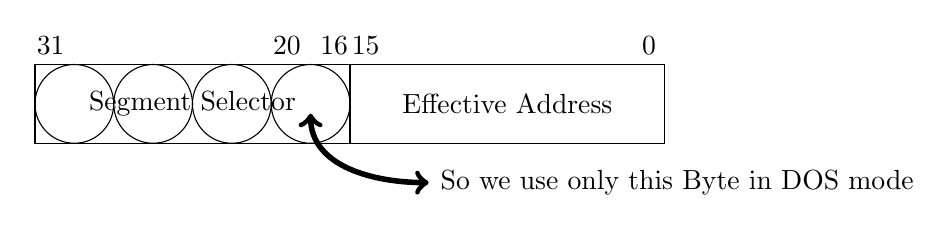
\begin{tikzpicture}
\coordinate [label=above:31] (A) at (0.2,1);
\coordinate [label=above:20] (A) at (3.2,1);
\coordinate [label=above:16] (A) at (3.8,1);
\coordinate [label=above:15] (A) at (4.2,1);
\coordinate [label=above:0] (A) at (7.8,1);
\draw (0,0) rectangle (4,1) node[pos=.5] {Segment Selector};
\draw (4,0) rectangle (8,1) node[pos=.5] {Effective Address};
\foreach \x in {1,2,3,4}
	\draw[baseline] (\x-0.5,0.5 ) node (N\x) {} circle (0.5);
\draw[<->,line width =2pt] [out=-90] (N4)  to [in=180] (5,-0.5) node[right]{So we use only this Byte in DOS mode} ;
\end{tikzpicture}
	
\end{center}
\end{note}

\begin{note}[Registers in real mode]: (p $\rightarrow$ 65)\\
\begin{center}
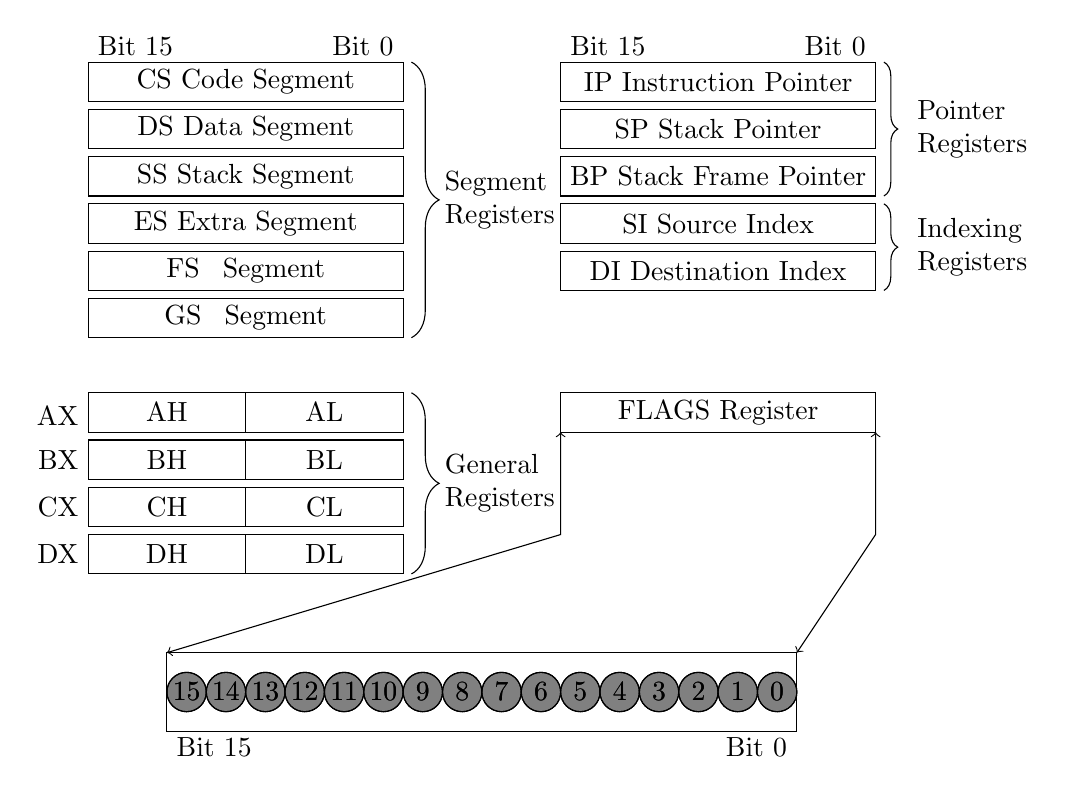
\begin{tikzpicture}
\node[left] at (0,0.25) {DX};
\draw (0,0) rectangle (2,.5) node [pos=0.5] {DH};
\draw (2,0) rectangle (4,.5) node [pos=0.5] {DL};

\node[left] at (0,0.85) {CX};
\draw (0,0.6) rectangle (2,1.1) node [pos=0.5] {CH};
\draw (2,0.6) rectangle (4,1.1) node [pos=0.5] {CL};

\node[left] at (0,1.45) {BX};
\draw (0,1.2) rectangle (2,1.7) node [pos=0.5] {BH};
\draw (2,1.2) rectangle (4,1.7) node [pos=0.5] {BL};

\node[left] at (0,2) {AX};
\draw (0,1.8) rectangle (2,2.3) node [pos=0.5] {AH};
\draw (2,1.8) rectangle (4,2.3) node [pos=0.5] {AL};

\draw [decorate,decoration={brace,amplitude=10pt,mirror},xshift=3pt,yshift=0pt]
(4,0) -- (4,2.3) node [black,midway,right,xshift=0.3cm,text width=1.5cm] 
{General Registers};

\draw (0,3) rectangle (4,3.5) node [pos=0.5] {GS \, Segment};
\draw (0,3.6) rectangle (4,4.1) node [pos=0.5] {FS \, Segment};
\draw (0,4.2) rectangle (4,4.7) node [pos=0.5] {ES Extra Segment};
\draw (0,4.8) rectangle (4,5.3) node [pos=0.5] {SS Stack Segment};
\draw (0,5.4) rectangle (4,5.9) node [pos=0.5] {DS Data Segment};
\draw (0,6) rectangle (4,6.5) node [pos=0.5] {CS Code Segment};

\draw [decorate,decoration={brace,amplitude=10pt,mirror},xshift=3pt,yshift=0pt]
(4,3) -- (4,6.5) node [black,midway,right,xshift=0.3cm,text width=1.5cm] 
{Segment Registers};

\node [right] at (0,6.7) {Bit 15};
\node [left] at (4,6.7) {Bit 0};

\draw (6,1.8) rectangle (10,2.3) node [pos=0.5] {FLAGS Register};

\draw (6,3.6) rectangle (10,4.1) node [pos=0.5] {DI Destination Index};
\draw (6,4.2) rectangle (10,4.7) node [pos=0.5] {SI Source Index};
\draw (6,4.8) rectangle (10,5.3) node [pos=0.5] {BP Stack Frame Pointer};
\draw (6,5.4) rectangle (10,5.9) node [pos=0.5] {SP Stack Pointer};
\draw (6,6) rectangle (10,6.5) node [pos=0.5] {IP Instruction Pointer};
\draw [decorate,decoration={brace,amplitude=5pt,mirror},xshift=3pt,yshift=0pt]
(10,4.8) -- (10,6.5) node [black,midway,right,xshift=0.3cm,text width=1.5cm] 
{Pointer Registers};
\draw [decorate,decoration={brace,amplitude=5pt,mirror},xshift=3pt,yshift=0pt]
(10,3.6) -- (10,4.7) node [black,midway,right,xshift=0.3cm,text width=1.5cm] 
{Indexing Registers};

\node [right] at (6,6.7) {Bit 15};
\node [left] at (10,6.7) {Bit 0};

\draw (1,-1) rectangle (9,-2);
\draw[<->] (6,1.8) -- (6,0.5) -- (1,-1);
\draw[<->] (10,1.8) -- (10,0.5) -- (9,-1);

\foreach \x in {15,...,0}
	\ifthenelse{9 = \x \OR  8 = \x}
	{\draw[fill=gray] (8-\x/2+.75,-1.5) node (B\x) {\x} circle (0.25);}
	{\draw (8-\x/2+.75,-1.5) node (B\x) {\x} circle (0.25);};

	
\node [right] at (1,-2.2) {Bit 15};
\node [left] at (9,-2.2) {Bit 0};
\end{tikzpicture}
\end{center}

\begin{itemize}
\item Bit 8 of FLAGS Register (TF Trap Flag): if this bit is set, the processor generates a single-step interrupt after each instruction. Debuggers use this to single-step through a program.
\item Bit 9 of FLAGS Register (IF Interrupt Enabled Flag): If it is set, then interrupts are enabled.
\end{itemize}
\end{note}

\begin{note}[Real-Mode Interrupts]
\begin{enumerate}
\item An interrupt is some event that triggers the execution of a special kind type of procedure called an \textit{interrupt service routine (ISR)}, also known as an \textit{interrupt handler}
\item In real mode, the first kilobyte of memory (address 0x00000 to 0x003FF) is occupied by \textit{interrupt vector table (IVT)}. In protected mode this structure is called \textit{interrupt descriptor table (IDT)}.
\item The logical address of each ISR in IVT is stored sequentially. like figure \ref{figRootKitRealModeIVT}.
\begin{center}
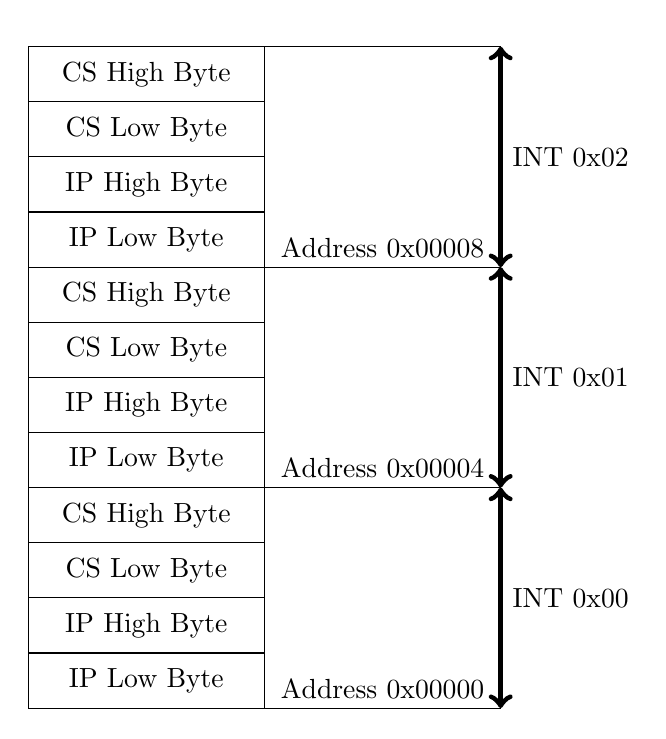
\begin{tikzpicture}
\label{figRootKitRealModeIVT}
\foreach \x in {0,2.8,5.6}
{
	\draw (0,\x) rectangle (3,\x+0.7) node [pos=0.5] {IP Low Byte};
	\draw (0,\x + 0.7) rectangle (3,\x+1.4) node [pos=0.5] {IP High Byte};	
	\draw (0,\x + 1.4) rectangle (3,\x+2.1) node [pos=0.5] {CS Low Byte};	
	\draw (0,\x + 2.1) rectangle (3,\x+2.8) node [pos=0.5] {CS High Byte};		
}
\draw (3,0) -- (6,0) node [pos = 0.5,above] {Address 0x00000};
\draw (3,2.8) -- (6,2.8) node [pos = 0.5,above] {Address 0x00004};
\draw (3,5.6) -- (6,5.6) node [pos = 0.5,above] {Address 0x00008};
\draw (3,8.4) -- (6,8.4) node [pos = 0.5,above] {};

\draw[<->, line width = 2pt] (6,0) -- (6,2.8) node [pos=0.5,right] {INT 0x00};
\draw[<->,line width = 2pt] (6,2.8) -- (6,5.6) node [pos=0.5,right] {INT 0x01};
\draw[<->,line width = 2pt] (6,5.6) -- (6,8.4) node [pos=0.5,right] {INT 0x02};
\end{tikzpicture}
\end{center}
\item Under MS-DOS, the BIOS handles interrupts 0 through 31, and DOS handles interrupts 32 through 63. the remaining interrupts (64 to 265) are for user-defined interrupts.
\item There are three types of Interrupts
\begin{itemize}
\item Hardware Interrupts (maskable and nonmaskable).
\item Software Interrupts.
\item Exceptions (faults, traps and aborts).
\end{itemize}
Maskbale hardware interrupts can be disabled by clearing IF\footnote{Interrupt Enabled Flag} like interrupt 8 (system timer). Software interrupts (also known as internal interrupts) are implemented in a program using INT instruction. like:
\begin{lstlisting} [language={[x86masm]Assembler}]
mov AH,02H
mov DL,41H
int 21H
\end{lstlisting}
\end{enumerate}
\end{note}

\begin{note}[Different jump types: Short, Near and Far:]\\

\begin{table}[!htbp]
	\makegapedcells
	\centering
	\resizebox{\textwidth}{!}{%resizing the whole table
\begin{tabular}{|c|c|c|}\hline
 \textbf{\textcolor{blue}{JMP Type}} & \textbf{\textcolor{blue}{Example}} & \textbf{\textcolor{blue}{Real Mode Machine Encoding}}  \\[\rowheight] \hline
\textbf{Short} & JMP SHORT mylabel & 0xEB [signed bytes]  \\ [\rowheight] \hline
\textbf{Near direct} & JMP NEAR PTR mylabel & 0xE9 [low byte][high byte]  \\ [\rowheight] \hline
\textbf{Near indirect} & JMP BX & 0xFF 0xE3  \\ [\rowheight] \hline
\textbf{Far direct} & JMP DS:[mylabel] & 0xEA [IP low][IP high][CS low][CS high]  \\ [\rowheight] \hline
\textbf{Far indirect} & JMP DWORD PTR [BX] & 0xFF 0x2F  \\ [\rowheight] \hline
 \textbf{\textcolor{blue}{CALL Type}} & \textbf{\textcolor{blue}{Example}} & \textbf{\textcolor{blue}{Real Mode Machine Encoding}}  \\[\rowheight] \hline
\textbf{Near direct} & CALL mylabel & 0xE8 [low byte][high byte]  \\ [\rowheight] \hline
\textbf{Near indirect} & CALL BX & 0xFF 0xD3  \\ [\rowheight] \hline
\textbf{Far direct} & CALL DS:[mylabel] & 0x9A [IP low][IP high][CS low][CS high]  \\ [\rowheight] \hline
\textbf{Far indirect} & CALL DWORD PTR [BX] & 0xFF 0x1F  \\ [\rowheight] \hline
\textbf{Near return} & RET & 0xC3  \\ [\rowheight] \hline
\textbf{Far return} & RETF & 0xCB  \\ [\rowheight] \hline
\end{tabular}
}
\caption{Jump and call tables}
\end{table}
\end{note}
\newpage
\section{Protected Mode (P.87)}
\begin{note}[Dedicated-purpose registers for protected mode]\\
\begin{center}
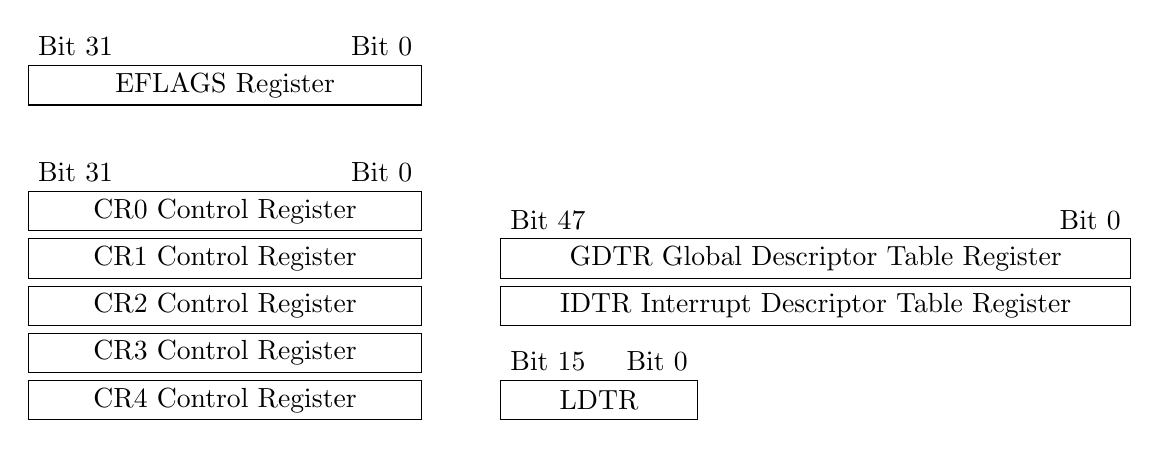
\begin{tikzpicture}
\draw (0,0) rectangle (5,0.5) node [pos=0.5] {CR4 Control Register};
\draw (0,0.6) rectangle (5,1.1) node [pos=0.5] {CR3 Control Register};
\draw (0,1.2) rectangle (5,1.7) node [pos=0.5] {CR2 Control Register};
\draw (0,1.8) rectangle (5,2.3) node [pos=0.5] {CR1 Control Register};
\draw (0,2.4) rectangle (5,2.9) node [pos=0.5] {CR0 Control Register};
\node at (0,2.9) [above right] {Bit 31};
\node at (5,2.9) [above left] {Bit 0};

\draw (0,4) rectangle (5,4.5) node [pos=0.5] {EFLAGS Register};
\node at (0,4.5) [above right] {Bit 31};
\node at (5,4.5) [above left] {Bit 0};

\draw (6,0) rectangle (8.5,0.5) node [pos=0.5] {LDTR};
\node at (6,0.5) [above right] {Bit 15};
\node at (8.5,0.5) [above left] {Bit 0};

\draw (6,1.2) rectangle (14,1.7) node [pos=0.5] {IDTR Interrupt Descriptor Table Register};
\draw (6,1.8) rectangle (14,2.3) node [pos=0.5] {GDTR Global Descriptor Table Register};
\node at (6,2.3) [above right] {Bit 47};
\node at (14,2.3) [above left] {Bit 0};
\end{tikzpicture}
\end{center}
\begin{itemize}
\item Of the six segment registers (CS,DS,ES,FS,GS,SS), the CS register is the only one that cannot be set explicitly. Instead, the CS Register contents must be set implicitly through instructions that transfer program control (JMP,CALL,INT,RET,IRET,SYSENTER,SYSEXIT,etc)
\end{itemize}
\end{note}

\begin{note}[Protected-Mode Segmentation]
\begin{itemize}
\item Paging is an optional feature but segmentation is mandatory.
\item There are two types of descriptor tables, GDT \footnote{Global Descriptor Table}  and LDT \footnote{Local Descriptor Table} , GDT is mandatory.
\remark \normalfont The first entry in GDT is always empty and is referred to as a \textit{null segment descriptor}. A selector that refers to this descriptor in the GDT is called \textit{null selector}.
\end{itemize}
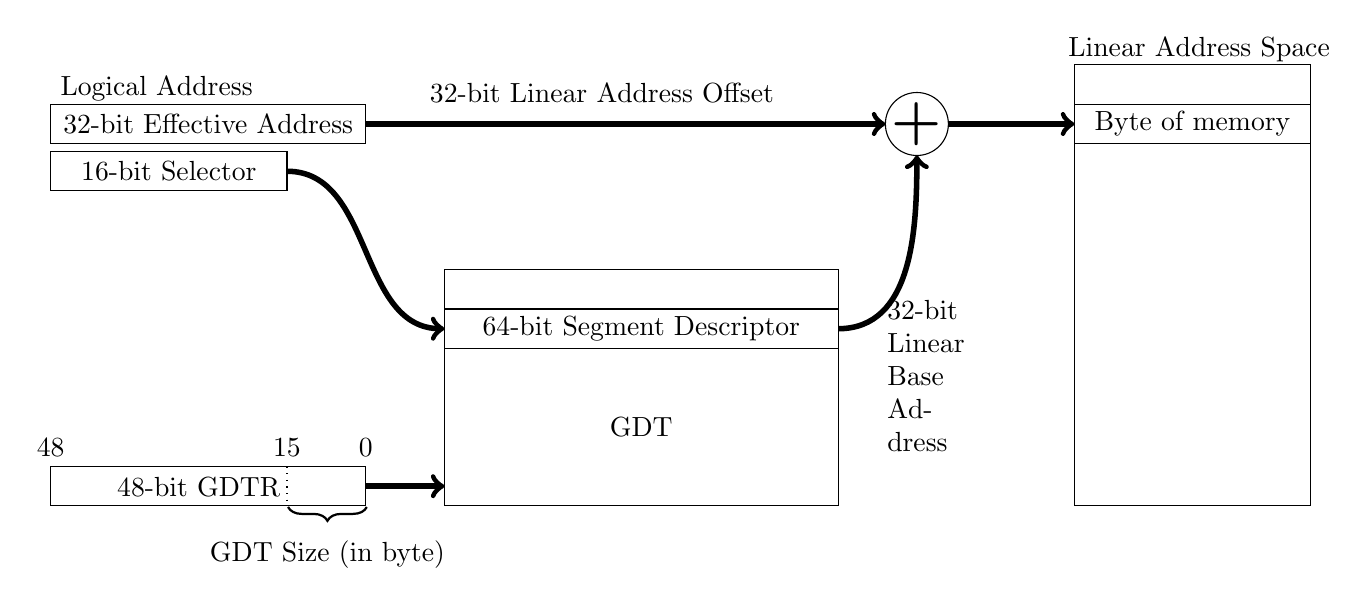
\begin{tikzpicture}
\draw (0,0) rectangle (4,0.5) node [pos=0.47] {48-bit GDTR};
\draw [thick,decorate,decoration={brace,amplitude=5pt,mirror},xshift=0.4pt,yshift=-0.4pt](3,0) -- (4,0) node[black,midway,yshift=-0.6cm] {GDT Size (in byte)};
\draw node at (0,0.5) [above] {48};
\draw node at (4,0.5) [above] {0};
\draw[dotted] (3,0.5) node [above] {15} -- (3,0);

\draw (5,0) rectangle (10,2) node [pos=0.5] {GDT};
\draw (5,2) rectangle (10,2.5) node [pos=0.5] {64-bit Segment Descriptor};
\draw (5,2.5) rectangle (10,3);

\draw (0,4) rectangle (3,4.5) node [pos=0.5] {16-bit Selector};
\draw (0,4.6) rectangle (4,5.1) node [pos=0.5] {32-bit Effective Address};
\draw node at (0,5.3) [above, right] {Logical Address} ;

\draw[->, line width = 2pt] [out = 0] (3,4.25) to [in = 180] (5,2.25);
\draw[->, line width = 2pt] [out = 0] (4,0.25) to [in = 180] (5,0.25);

\draw (11,4.85) circle (0.4) node {\textbf{\huge +}};
\draw[->, line width = 2pt] [out = 0] (4,4.85) to [in = 180] (10.6,4.85) ;
\draw node at (7,5) [above] {32-bit Linear Address Offset} ;
\draw[->, line width = 2pt] [out = 0] (10,2.25) to [in = -90] (11,4.45);
\draw node at (10.5,1.65) [right,text width=1.2cm] {32-bit Linear Base Address} ;

\draw (13,0) rectangle (16,4.6);
\draw (13,4.6) rectangle (16,5.1) node [pos=0.5] {Byte of memory};
\draw (13,5.1) rectangle (16,5.6);
\draw node at (12.8,5.8) [above, right] {Linear Address Space} ;
\draw[->, line width = 2pt] [out = 0] (11.4,4.85) to [in = 180] (13,4.85);
\end{tikzpicture}\\

The most 13 valuable bits of the Segment Selector are index into GDT. So there can be only $2^{13} = 8192$ entries, and each entry (Segment Descriptor) is 8 byte long so maximum size of GDT is $2^{13} \times 2^{3} = 2^{16}$ in byte which perfectly fits into GDTR size partition.

\begin{center}
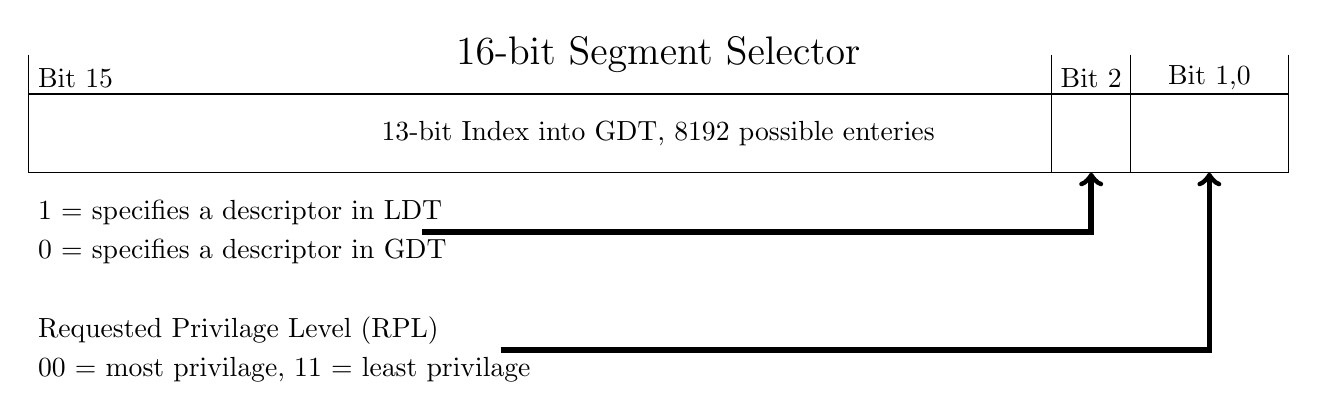
\begin{tikzpicture}
\draw node at (8,1.5) {{\Large 16-bit Segment Selector}};
\draw (0,0)  rectangle (16,1) node [pos=0.5] {13-bit Index into GDT, 8192 possible enteries};
\foreach \x in {16,14,13,0}
\draw (\x,1.5) -- (\x,0);
\draw node at (15,1.2) {Bit 1,0};
\draw node at (13.5,1.2) {Bit 2};
\draw node at (0,1.2) [right] {Bit 15};
\draw node at (0,-0.5) [right] {1 = specifies a descriptor in LDT};
\draw node at (0,-1) [right] {0 = specifies a descriptor in GDT};
\draw node at (0,-2) [right] {Requested Privilage Level (RPL)};
\draw node at (0,-2.5) [right] {00 = most privilage, 11 = least privilage};
\draw[->, line width = 2pt] (5,-0.75) -- (13.5,-0.75) -- (13.5,0);
\draw[->, line width = 2pt] (6,-2.25) -- (15,-2.25) -- (15,0);
\end{tikzpicture}
\end{center}

So the the instruction
\lstinline [language={[x86masm]Assembler}] {mov FS:[30h], 0}
When Linear Base Address referenced by FS is 0x00100000, is to
\lstinline [language={[x86masm]Assembler}] {mov [100030h], 0}. Note that in this design, some over allowed Linear Addresses can be generated, for example if Effective Address was 0x20000000 and the Linear Base Address was 0xEFFFFFFF, the result would be greater than 0xFFFFFFFF which is the summit of the 32-bit address space.
\begin{itemize}
\item There are two specific instructions to work with GDTR, The LGDT loads a value into GDTR and the SGDT reads the value stored in GDTR.
\item RPL \footnote{Requested Privilege Level} is stored in Segment Selectors, DPL \footnote{Descriptor Privilege Level} is kept in Segment Descriptors.A Segment with a DPL of 0 is referred to as existing inside of Ring 0. The CPL or \textit{Current Privilege Level} is the value of RPL in the CS and SS Registers.
\end{itemize}
\begin{center}
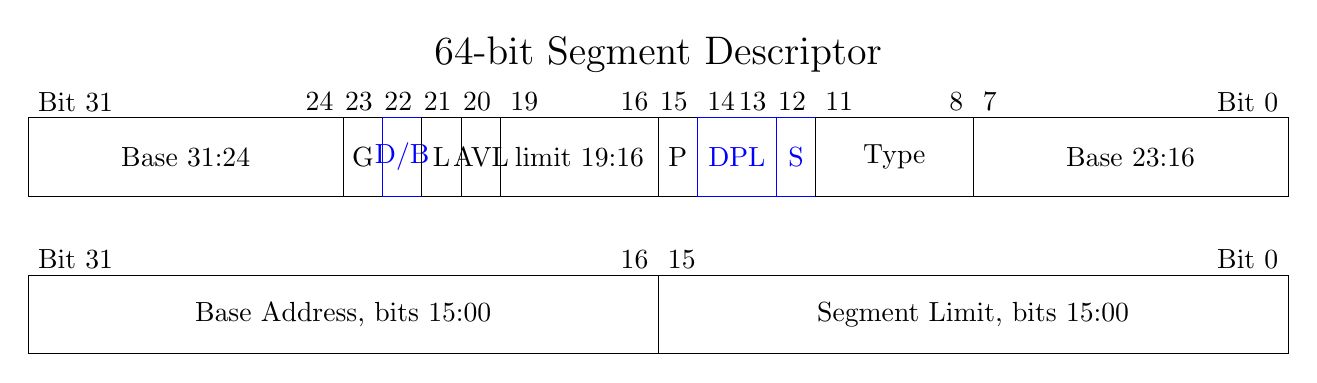
\begin{tikzpicture}
\draw node at (8,3.8) {{\Large 64-bit Segment Descriptor}};
\draw (0,2)  rectangle (4,3) node [pos=0.5] {Base 31:24}; \draw node at (0,3.2) [right] {Bit 31};
\draw (4,2)  rectangle (4.5,3) node [pos=0.5] {G}; \draw node at (4,3.2) [left] {24};
\draw [blue] (4.5,2)  rectangle (5,3) node [pos=0.5] {D/B};\draw node at (4.5,3.2) [left] {23};
\draw (5,2)  rectangle (5.5,3) node [pos=0.5] {L};\draw node at (5,3.2) [left] {22};
\draw (5.5,2)  rectangle (6,3) node [pos=0.5] {AVL}; \draw node at (5.5,3.2) [left] {21};
\draw (6,2)  rectangle (8,3) node [pos=0.5] {limit 19:16}; \draw node at (6,3.2) [left] {20}; \draw node at (6,3.2) [right] {19};
\draw (8,2)  rectangle (8.5,3) node [pos=0.5] {P}; \draw node at (8,3.2) [left] {16};
\draw [blue] (8.5,2)  rectangle (9.5,3) node [pos=0.5] {DPL};\draw node at (8.5,3.2) [left] {15}; \draw node at (8.5,3.2) [right] {14};
\draw [blue] (9.5,2) rectangle (10,3) node [pos=0.5] {S};\draw node at (9.5,3.2) [left] {13};
\draw (10,2)  rectangle (12,3) node [pos=0.5] {Type}; \draw node at (10,3.2) [left] {12}; \draw node at (10,3.2) [right] {11};
\draw (12,2)  rectangle (16,3) node [pos=0.5] {Base 23:16};\draw node at (12,3.2) [left] {8};
\draw (0,0)  rectangle (8,1) node [pos=0.5] {Base Address, bits 15:00};\draw node at (12,3.2) [right] {7};
\draw (8,0)  rectangle (16,1) node [pos=0.5] {Segment Limit, bits 15:00};
\draw node at (16,1.2) [left] {Bit 0};
\draw node at (8,1.2) [right] {15};
\draw node at (8,1.2) [left] {16};
\draw node at (0,1.2) [right] {Bit 31};
\draw node at (16,3.2) [left] {Bit 0};
\end{tikzpicture}

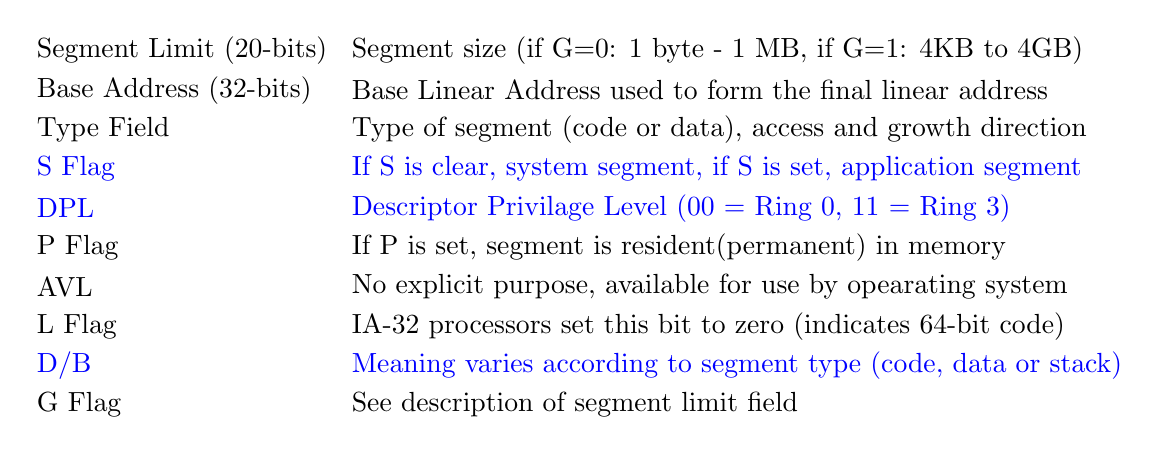
\begin{tikzpicture}
\draw node at (0,-0.5) [right] {Segment Limit (20-bits)};
\draw node at (0,-1) [right] {Base Address (32-bits)};
\draw node at (0,-1.5) [right] {Type Field};
\draw [blue] node at (0,-2) [right] {S Flag};
\draw [blue] node at (0,-2.5) [right] {DPL};
\draw node at (0,-3) [right] {P Flag};
\draw node at (0,-3.5) [right] {AVL};
\draw node at (0,-4) [right] {L Flag};
\draw [blue] node at (0,-4.5) [right] {D/B};
\draw node at (0,-5) [right] {G Flag};

\draw node at (4,-0.5) [right] {Segment size (if G=0: 1 byte - 1 MB, if G=1: 4KB to 4GB)};
\draw node at (4,-1) [right] {Base Linear Address used to form the final linear address};
\draw node at (4,-1.5) [right] {Type of segment (code or data), access and growth direction};
\draw [blue] node at (4,-2) [right] {If S is clear, system segment, if S is set, application segment};
\draw [blue] node at (4,-2.5) [right] {Descriptor Privilage Level (00 = Ring 0, 11 = Ring 3)};
\draw node at (4,-3) [right] {If P is set, segment is resident(permanent) in memory};
\draw node at (4,-3.5) [right] {No explicit purpose, available for use by opearating system};
\draw node at (4,-4) [right] {IA-32 processors set this bit to zero (indicates 64-bit code)};
\draw [blue] node at (4,-4.5) [right] {Meaning varies according to segment type (code, data or stack)};
\draw node at (4,-5) [right] {See description of segment limit field};
\end{tikzpicture}
\end{center}
\end{note}

\begin{note}[Protected-Mode Paging]
\begin{itemize}
\item Each page can be 4KB, 2MB or 4MB in size.
\item If a program references a byte in a page of memory that's currently stored on disk, the processor will generate a \textit{page fault \#PF} exception.
\item The slot in physical memory which pages will be loaded into is called a \textit{page frame}.
\item 32-bit linear address under paging
\begin{center}
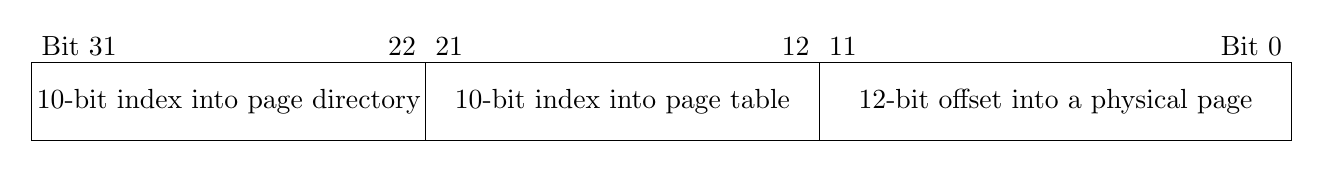
\begin{tikzpicture}
\draw (0,0) rectangle (5,1) node [pos=0.5] {10-bit index into page directory};
\draw (5,0) rectangle (10,1) node [pos=0.5] {10-bit index into page table};
\draw (10,0) rectangle (16,1) node [pos=0.5] {12-bit offset into a physical page};
\draw node at (0,1.2) [right] {Bit 31};
\draw node at (5,1.2) [left] {22};
\draw node at (5,1.2) [right] {21};
\draw node at (10,1.2) [left] {12};
\draw node at (10,1.2) [right] {11};
\draw node at (16,1.2) [left] {Bit 0};
\end{tikzpicture}
\end{center}
\item The physical address (not the linear address) of the first entry of the \textit{page directory} is stored in control register \textbf{CR3}.
\item Each PDE \footnote{Page Directory Entry} contains the base physical address (not the linear address) of a secondary array structure known as the \textit{page table}.
\item Each PTE \footnote{Page Table Entry} contains the physical address of a page of memory.
\end{itemize}
\begin{center}
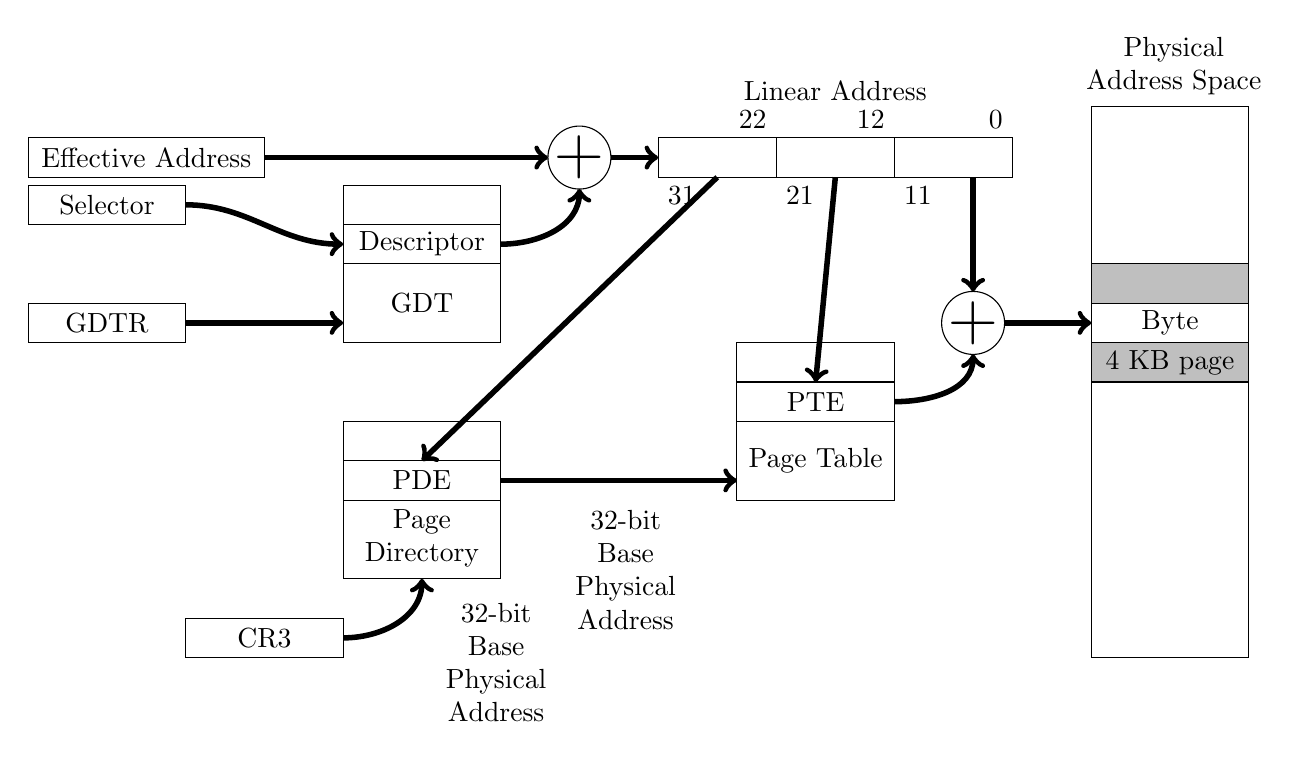
\begin{tikzpicture}
\draw (2,0) rectangle (4,0.5) node [pos=0.5] {CR3};
\draw[->,line width = 2pt] [out=0] (4,0.25) to [in = -90](5,1) node [label={[align=center]-45:32-bit \\Base \\Physical\\ Address}] {};
\draw (4,1) rectangle (6,2) node [label={[align=center,xshift=-1.0cm, yshift=-1.1cm]Page\\Directory}] {};
\draw (4,2) rectangle (6,2.5) node [pos = 0.5] {PDE};
\draw[->,line width=2pt] (6,2.25) -- (9,2.25) node [label={[align=center,label distance = 0.5cm]-160:32-bit \\Base \\Physical\\ Address}] {};
\draw (4,2.5) rectangle (6,3);

\draw (0,4) rectangle (2,4.5) node [pos=0.5] {GDTR};
\draw [->,line width = 2pt] (2,4.25) to (4,4.25);
\draw (4,4) rectangle (6,5) node [pos=0.5] {GDT};
\draw (4,5) rectangle (6,5.5) node [pos = 0.5] {Descriptor};
\draw [->,line width = 2pt,out = 0] (6,5.25) to [in = -90] (7,5.95);
\draw (4,5.5) rectangle (6,6);

\draw (0,5.5) rectangle (2,6) node [pos=0.5] {Selector};
\draw [->,line width = 2pt,out = 0] (2,5.75) to [in = 180] (4,5.25);
\draw (0,6.1) rectangle (3,6.6) node [pos=0.5] {Effective Address};
\draw [->,line width = 2pt] (3,6.35) to (6.6,6.35);
\draw (7,6.35) circle (0.4) node {\Huge +};
\draw [->,line width = 2pt] (7.4,6.35) to (8,6.35);

\draw (8,6.1) node [below right] {31} rectangle (9.5,6.6) node [above left] {22};
\draw [->,line width = 2pt] (8.75,6.1) to (5,2.5);
\draw (9.5,6.1) node [below right] {21} rectangle (11,6.6) node [above left] {12};
\draw [->,line width = 2pt] (10.25,6.1) to (10,3.5);
\draw (11,6.1) node [below right] {11} rectangle (12.5,6.6) node [above left] {0};
\draw node at (10.25,7.2) {Linear Address};

\draw (9,2) rectangle (11,3) node [pos=0.5] {Page Table};
\draw (9,3) rectangle (11,3.5) node [pos = 0.5] {PTE};
\draw (9,3.5) rectangle (11,4);

\draw (13.5,0) rectangle (15.5,3.5);
\draw[fill=lightgray] (13.5,3.5) rectangle (15.5,4) node [pos=0.5] {4 KB page};
\draw (13.5,4) rectangle (15.5,4.5) node [pos=0.5] {Byte};
\draw[fill=lightgray] (13.5,4.5) rectangle (15.5,5);
\draw (13.5,4.5) rectangle (15.5,7);
\draw node at (14.25,7.5) [label={[align=center,xshift=0.3cm,yshift=-0.6cm]Physical \\Address Space}] {};

\draw (12,4.25) circle (0.4) node {\Huge +};
\draw [->,line width = 2pt] (12,6.1) to (12,4.65);
\draw [->,line width = 2pt] (12.4,4.25) to (13.5,4.25);
\draw [->,line width = 2pt, out = 0] (11,3.25) to [in = -90] (12,3.85);
\end{tikzpicture}
\end{center}

With the described routine of paging, we are restricted to 4GB of memory ($1024 \times 1024 \times 4096 = 4GB$). But with the assistive method of PAE\footnote{Paging with Address Extension} we can extend the limit up to 52 address lines.
\end{note}

\begin{note}[Paging with Address Extension (PAE)]
\begin{enumerate}
\item There is a PAE flag in CR4 which PAE is enabled if that flag is set.
\item With PAE enabled, the linear address is broken into four parts instead of just three.
\begin{center}
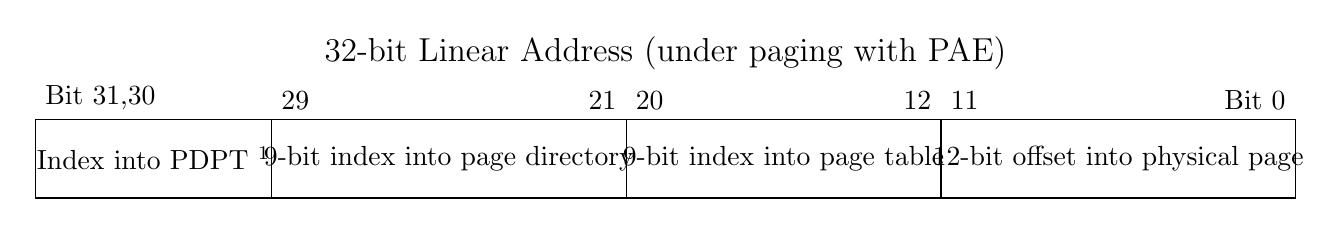
\begin{tikzpicture}
\draw (0,0) rectangle (3,1) node [pos = 0.5] {Index into PDPT \footnote{Page Directory Pointer Table}};
\draw (3,0) rectangle (7.5,1) node [pos = 0.5] {9-bit index into page directory};
\draw (7.5,0) rectangle (11.5,1) node [pos = 0.5] {9-bit index into page table};
\draw (11.5,0) rectangle (16,1) node [pos = 0.5] {12-bit offset into physical page};
\draw node at (0,1) [above right] {Bit 31,30};
\draw node at (3,1) [above right] {29};
\draw node at (7.5,1) [above left] {21};
\draw node at (7.5,1) [above right] {20};
\draw node at (11.5,1) [above left] {12};
\draw node at (11.5,1) [above right] {11};
\draw node at (16,1) [above left] {Bit 0};
\draw node at (8,1.5) [above] {{\large 32-bit Linear Address (under paging with PAE)}};
\end{tikzpicture}
\end{center}
\item Paging with PAE maps a 32-bit linear address to a 52-bit physical address. If a particular IA-32 processor has less than 52 address lines, the corresponding higher order bits of each physical address generated will simply set to zero.
\item Take a look at image on P $\rightarrow$ 97
\end{enumerate}
\end{note}

\begin{note}[A Closer Look at the Tables]
\begin{itemize}
\item Both the PDE and PTE are 32-bit structures.
\end{itemize}
\begin{center}
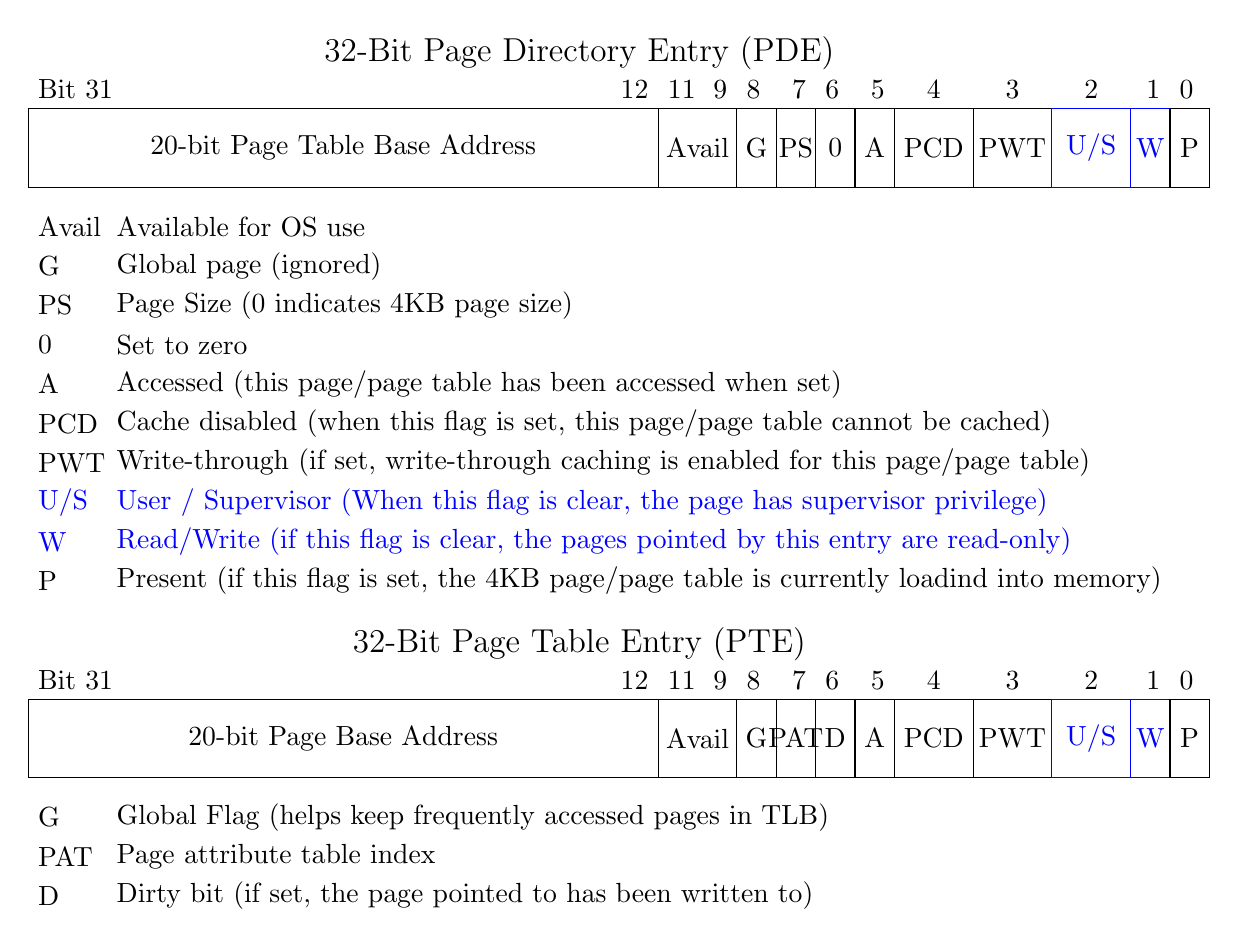
\begin{tikzpicture}
\draw node at (7,1.7) {{\large 32-Bit Page Directory Entry (PDE)}};
\draw (0,0) rectangle (8,1) node [pos = 0.5] {20-bit Page Table Base Address};
\draw (8,0) rectangle (9,1) node [pos = 0.5] {Avail};
\draw (9,0) rectangle (9.5,1) node [pos = 0.5] {G};
\draw (9.5,0) rectangle (10,1) node [pos = 0.5] {PS};
\draw (10,0) rectangle (10.5,1) node [pos = 0.5] {0};
\draw (10.5,0) rectangle (11,1) node [pos = 0.5] {A};
\draw (11,0) rectangle (12,1) node [pos = 0.5] {PCD};
\draw (12,0) rectangle (13,1) node [pos = 0.5] {PWT};
\draw [blue] (13,0) rectangle (14,1) node [pos = 0.5] {U/S};
\draw [blue] (14,0) rectangle (14.5,1) node [pos = 0.5] {W};
\draw (14.5,0) rectangle (15,1) node [pos = 0.5] {P};

\draw node at (0,1) [above right] {Bit 31};
\draw node at (8,1) [above left] {12};
\draw node at (8,1) [above right] {11};
\draw node at (9,1) [above left] {9};
\draw node at (9,1) [above right] {8};
\draw node at (10,1) [above left] {7};
\draw node at (10,1) [above right] {6};
\draw node at (11,1) [above left] {5};
\draw node at (11.5,1) [above] {4};
\draw node at (12.5,1) [above] {3};
\draw node at (13.5,1) [above] {2};
\draw node at (14.5,1) [above left] {1};
\draw node at (14.5,1) [above right] {0};

\draw node at (0,-0.5) [right] {Avail};
\draw node at (1,-0.5) [right] {Available for OS use};
\draw node at (0,-1) [right] {G};
\draw node at (1,-1) [right] {Global page (ignored)};
\draw node at (0,-1.5) [right] {PS};
\draw node at (1,-1.5) [right] {Page Size (0 indicates 4KB page size)};
\draw node at (0,-2) [right] {0};
\draw node at (1,-2) [right] {Set to zero};
\draw node at (0,-2.5) [right] {A};
\draw node at (1,-2.5) [right] {Accessed (this page/page table has been accessed when set)};
\draw node at (0,-3) [right] {PCD};
\draw node at (1,-3) [right] {Cache disabled (when this flag is set, this page/page table cannot be cached)};
\draw node at (0,-3.5) [right] {PWT};
\draw node at (1,-3.5) [right] {Write-through (if set, write-through caching is enabled for this page/page table)};
\draw [blue] node at (0,-4) [right] {U/S};
\draw [blue] node at (1,-4) [right] {User / Supervisor (When this flag is clear, the page has supervisor privilege)};
\draw [blue] node at (0,-4.5) [right] {W};
\draw [blue] node at (1,-4.5) [right] {Read/Write (if this flag is clear, the pages pointed by this entry are read-only)};
\draw node at (0,-5) [right] {P};
\draw node at (1,-5) [right] {Present (if this flag is set, the 4KB page/page table is currently loadind into memory)};

\draw node at (7,-5.8) {{\large 32-Bit Page Table Entry (PTE)}};
\draw (0,-7.5) rectangle (8,-6.5) node [pos = 0.5] {20-bit Page Base Address};
\draw (8,-7.5) rectangle (9,-6.5) node [pos = 0.5] {Avail};
\draw (9,-7.5) rectangle (9.5,-6.5) node [pos = 0.5] {G};
\draw (9.5,-7.5) rectangle (10,-6.5) node [pos = 0.5] {PAT};
\draw (10,-7.5) rectangle (10.5,-6.5) node [pos = 0.5] {D};
\draw (10.5,-7.5) rectangle (11,-6.5) node [pos = 0.5] {A};
\draw (11,-7.5) rectangle (12,-6.5) node [pos = 0.5] {PCD};
\draw (12,-7.5) rectangle (13,-6.5) node [pos = 0.5] {PWT};
\draw [blue] (13,-7.5) rectangle (14,-6.5) node [pos = 0.5] {U/S};
\draw [blue] (14,-7.5) rectangle (14.5,-6.5) node [pos = 0.5] {W};
\draw (14.5,-7.5) rectangle (15,-6.5) node [pos = 0.5] {P};

\draw node at (0,-6.5) [above right] {Bit 31};
\draw node at (8,-6.5) [above left] {12};
\draw node at (8,-6.5) [above right] {11};
\draw node at (9,-6.5) [above left] {9};
\draw node at (9,-6.5) [above right] {8};
\draw node at (10,-6.5) [above left] {7};
\draw node at (10,-6.5) [above right] {6};
\draw node at (11,-6.5) [above left] {5};
\draw node at (11.5,-6.5) [above] {4};
\draw node at (12.5,-6.5) [above] {3};
\draw node at (13.5,-6.5) [above] {2};
\draw node at (14.5,-6.5) [above left] {1};
\draw node at (14.5,-6.5) [above right] {0};

\draw node at (0,-8) [right] {G};
\draw node at (1,-8) [right] {Global Flag (helps keep frequently accessed pages in TLB)};
\draw node at (0,-8.5) [right] {PAT};
\draw node at (1,-8.5) [right] {Page attribute table index};
\draw node at (0,-9) [right] {D};
\draw node at (1,-9) [right] {Dirty bit (if set, the page pointed to has been written to)};
\end{tikzpicture}
\end{center}
Implicit zeros will be added to each Base Address to turn those into 32-bit addresses.
\end{note}

\begin{note}[A Closer Look at the Control Registers]
\begin{enumerate}
\item If each process is given it's own copy of CR3, as part of its scheduling context, then it would be possible for two process to have the same linear address and yet have that linear address map to a different physical address.
\item CR0's 16th bit is a WP flag (as in write protection). When the WP is set, supervisor level code is not allowed to write into read-only user level memory pages. Whereas this mechanism facilitates the copy-on-write method of process creation (i.e., forking) traditionally used by UNIX systems, this is dangerous to us because it means that a rootkit might not be able to modify certain system data structures.
\end{enumerate}

\begin{center}
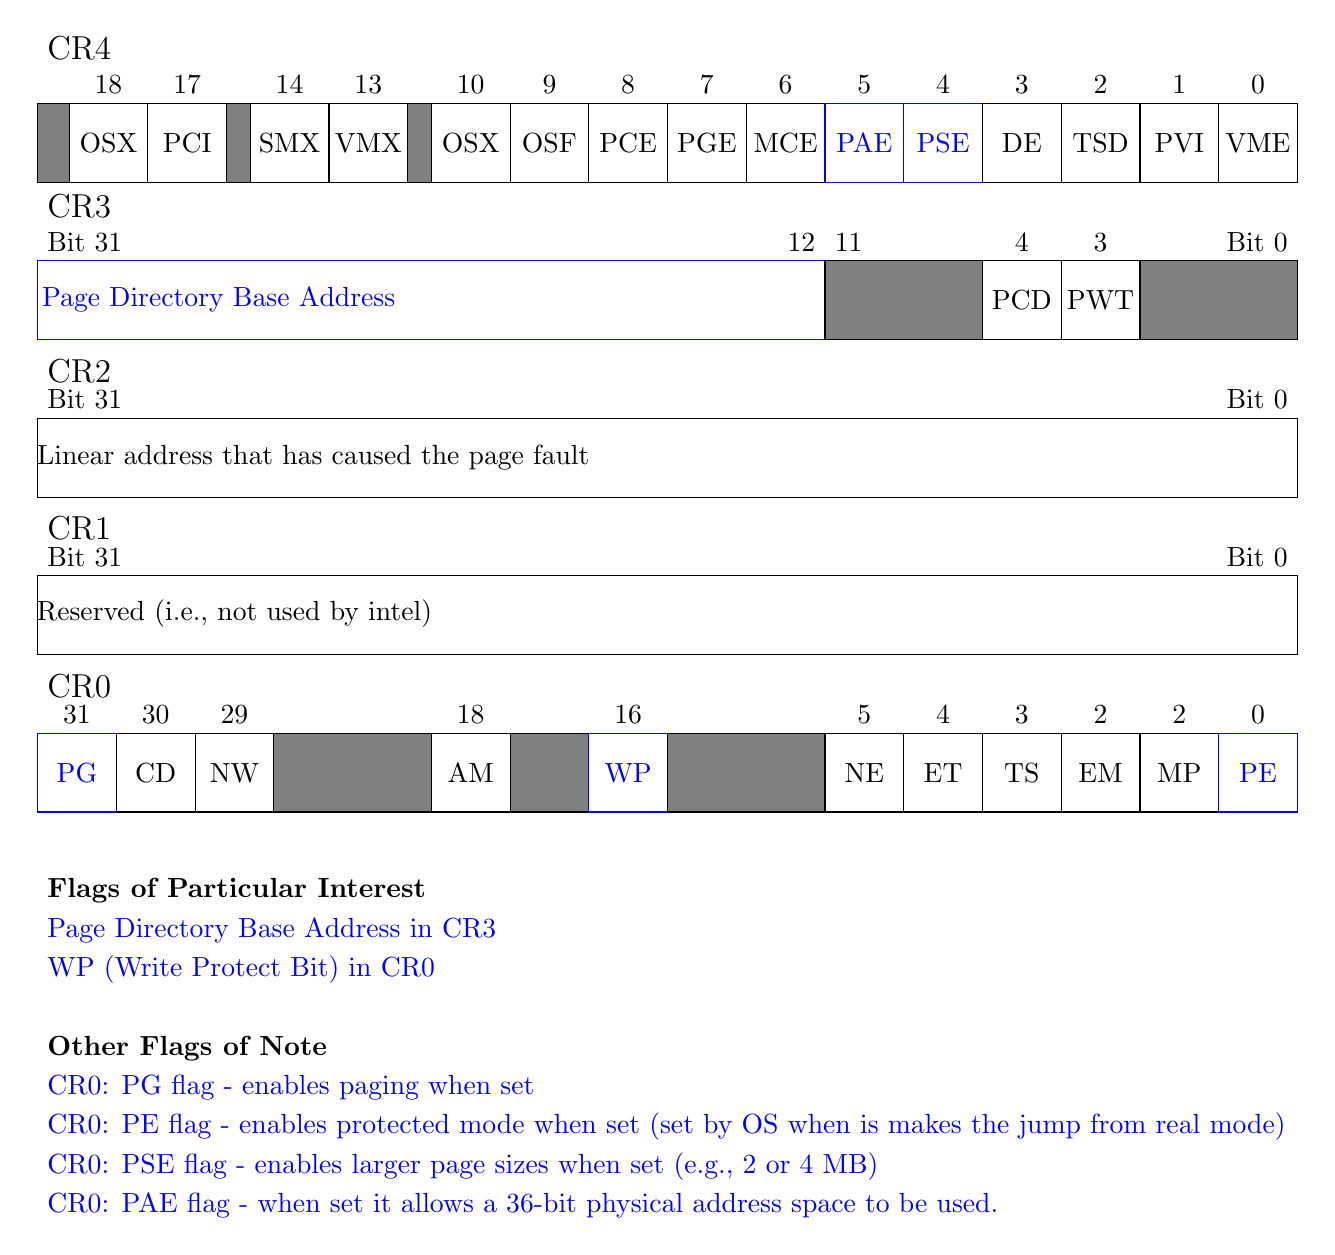
\begin{tikzpicture}
\draw [blue] (0,0) rectangle (1,1) node [pos=0.5] {PG}; \draw node at (0.5,1) [above] {31};
\draw (1,0) rectangle (2,1) node [pos=0.5] {CD}; \draw node at (1.5,1) [above] {30};
\draw (2,0) rectangle (3,1) node [pos=0.5] {NW}; \draw node at (2.5,1) [above] {29};
\draw [fill=gray] (3,0) rectangle (5,1);
\draw (5,0) rectangle (6,1) node [pos=0.5] {AM}; \draw node at (5.5,1) [above] {18};
\draw [fill=gray] (6,0) rectangle (7,1);
\draw [blue] (7,0) rectangle (8,1) node [pos=0.5] {WP}; \draw node at (7.5,1) [above] {16};
\draw [fill=gray] (8,0) rectangle (10,1);
\draw (10,0) rectangle (11,1) node [pos=0.5] {NE}; \draw node at (10.5,1) [above] {5};
\draw (11,0) rectangle (12,1) node [pos=0.5] {ET}; \draw node at (11.5,1) [above] {4};
\draw (12,0) rectangle (13,1) node [pos=0.5] {TS}; \draw node at (12.5,1) [above] {3};
\draw (13,0) rectangle (14,1) node [pos=0.5] {EM}; \draw node at (13.5,1) [above] {2};
\draw (14,0) rectangle (15,1) node [pos=0.5] {MP}; \draw node at (14.5,1) [above] {2};
\draw [blue] (15,0) rectangle (16,1) node [pos=0.5] {PE}; \draw node at (15.5,1) [above] {0};
\draw node at (0,1.6) [right] {\large CR0};

\draw (0,2) rectangle (16,3) node [label={[align=center,xshift=-13.5cm, yshift=-0.9cm] Reserved (i.e., not used by intel)}] {};
\draw node at (0,3) [above right] {Bit 31};
\draw node at (16,3) [above left] {Bit 0};
\draw node at (0,3.6) [right] {\large CR1};

\draw (0,4) rectangle (16,5) node [label={[align=center,xshift=-12.5cm, yshift=-0.9cm] Linear address that has caused the page fault}] {};
\draw node at (0,5) [above right] {Bit 31};
\draw node at (16,5) [above left] {Bit 0};
\draw node at (0,5.6) [right] {\large CR2};

\draw [blue] (0,6) rectangle (10,7) node [label={[align=center,xshift=-7.7cm, yshift=-0.9cm] Page Directory Base Address}] {};
\draw [fill=gray] (10,6) rectangle (12,7);
\draw node at (10,7) [above left] {12}; \draw node at (10,7) [above right] {11};
\draw (12,6) rectangle (13,7) node [pos=0.5] {PCD}; \draw node at (12.5,7) [above] {4};
\draw (13,6) rectangle (14,7) node [pos=0.5] {PWT}; \draw node at (13.5,7) [above] {3};
\draw [fill=gray] (14,6) rectangle (16,7);
\draw node at (0,7) [above right] {Bit 31};
\draw node at (16,7) [above left] {Bit 0};
\draw node at (0,7.7) [right] {\large CR3};

\draw [fill=gray] (0,8) rectangle (0.4,9);
\draw (0.4,8) rectangle (1.4,9) node [pos=0.5] {OSX}; \draw node at (0.9,9) [above] {18};
\draw (1.4,8) rectangle (2.4,9) node [pos=0.5] {PCI}; \draw node at (1.9,9) [above] {17};
\draw [fill=gray] (2.4,8) rectangle (2.7,9);
\draw (2.7,8) rectangle (3.7,9) node [pos=0.5] {SMX}; \draw node at (3.2,9) [above] {14};
\draw (3.7,8) rectangle (4.7,9) node [pos=0.5] {VMX}; \draw node at (4.2,9) [above] {13};
\draw [fill=gray] (4.7,8) rectangle (5,9);
\draw (5,8) rectangle (6,9) node [pos=0.5] {OSX}; \draw node at (5.5,9) [above] {10};
\draw (6,8) rectangle (7,9) node [pos=0.5] {OSF}; \draw node at (6.5,9) [above] {9};
\draw (7,8) rectangle (8,9) node [pos=0.5] {PCE}; \draw node at (7.5,9) [above] {8};
\draw (8,8) rectangle (9,9) node [pos=0.5] {PGE}; \draw node at (8.5,9) [above] {7};
\draw (9,8) rectangle (10,9) node [pos=0.5] {MCE}; \draw node at (9.5,9) [above] {6};
\draw [blue] (10,8) rectangle (11,9) node [pos=0.5] {PAE}; \draw node at (10.5,9) [above] {5};
\draw [blue] (11,8) rectangle (12,9) node [pos=0.5] {PSE}; \draw node at (11.5,9) [above] {4};
\draw (12,8) rectangle (13,9) node [pos=0.5] {DE}; \draw node at (12.5,9) [above] {3};
\draw (13,8) rectangle (14,9) node [pos=0.5] {TSD}; \draw node at (13.5,9) [above] {2};
\draw (14,8) rectangle (15,9) node [pos=0.5] {PVI}; \draw node at (14.5,9) [above] {1};
\draw (15,8) rectangle (16,9) node [pos=0.5] {VME}; \draw node at (15.5,9) [above] {0};
\draw node at (0,9.7) [right] {\large CR4};

\draw node at (0,-1) [right] {\textbf{Flags of Particular Interest}};
\draw [blue] node at (0,-1.5) [right] {Page Directory Base Address in CR3};
\draw [blue] node at (0,-2) [right] {WP (Write Protect Bit) in CR0};
\draw node at (0,-3) [right] {\textbf{Other Flags of Note}};
\draw [blue] node at (0,-3.5) [right] {CR0: PG flag - enables paging when set};
\draw [blue] node at (0,-4) [right] {CR0: PE flag - enables protected mode when set (set by OS when is makes the jump from real mode)};
\draw [blue] node at (0,-4.5) [right] {CR0: PSE flag - enables larger page sizes when set (e.g., 2 or 4 MB)};
\draw [blue] node at (0,-5) [right] {CR0: PAE flag - when set it allows a 36-bit physical address space to be used.};
\end{tikzpicture}
\end{center}
\end{note}
\section{Implementing Memory Protection (Chapter 3.5) P $\rightarrow $102}
\begin{note}[Protection Through Segmentation]
The following checks are performed:
\begin{itemize}
\item Limit checks.
\item Segment-type checks
\item Privilege-level checks.
\item Restricted instruction checks.
\end{itemize}
All of these checks will occur before the memory access cycle begins. If a violation occurs, a general-protection exception (often denoted by \#GP) will be generated by the processor.
\end{note}

\begin{note}[Segmentation Protection : Limit Checks]
\begin{enumerate}
\item Using 20-bit limit field of segment descriptors (in GDT or LDT) to ensure the program does not access the memory that isn't there.
\item Using GDTR's size limit to not allow access of entries that lie outside of GDT
\end{enumerate}
\end{note}
\chapter{UEFI, BIOS and platform}
\begin{note}[Abbreviations]:\\
	\begin{table}[h]
	\makegapedcells
	\centering
	\resizebox{\textwidth}{!}{%resizing the whole table
\begin{tabular}{|c|P{13cm}|}\hline
\textbf{Abbreviation} & \textbf{Meaning} \\  \hline

\href{https://en.wikipedia.org/wiki/Advanced_Configuration_and_Power_Interface}{\textbf{ACPI}} & Advanced Configuration and Power Interface \\   \hline
\href{https://en.wikipedia.org/wiki/Advanced_Programmable_Interrupt_Controller}{\textbf{APIC}} & Advanced Programmable Interrupt Controller \\   \hline
\href{https://en.wikipedia.org/wiki/Direct_memory_access}{\textbf{DMA}} & Direct Memory Access \\   \hline
\href{https://en.wikipedia.org/wiki/Direct_Media_Interface}{\textbf{DMI}} & Direct Media Interface \\   \hline
\href{https://en.wikipedia.org/wiki/EFI_system_partition}{\textbf{ESP}} & EFI System Partition \\   \hline
\href{https://www.dataman.com/media/datasheet/Intel/82802Ax.pdf}{\textbf{FWH}} & Firmware Hub \\   \hline
\href{https://en.wikipedia.org/wiki/GUID_Partition_Table}{\textbf{GPT}} & GUID Partition Table \\   \hline
\href{https://en.wikipedia.org/wiki/I/O_Controller_Hub}{\textbf{ICH}} & I/O Controller Hub (Southbridge)\\   \hline
\href{https://en.wikipedia.org/wiki/Industry_Standard_Architecture}{\textbf{ISA}} & Industry Standard Architecture\\   \hline
\href{https://en.wikipedia.org/wiki/Low_Pin_Count}{\textbf{LPC}} & Low Pin Count \\   \hline
\href{https://en.wikipedia.org/wiki/Northbridge_(computing)}{\textbf{MCH}} & Memory Controller Hub (Northbridge)\\   \hline
\href{https://en.wikipedia.org/wiki/Platform_Controller_Hub}{\textbf{PCH}} & Platform Controller Hub\\   \hline
\href{https://en.wikipedia.org/wiki/Conventional_PCI}{\textbf{PCI}} & Peripheral Component Interconnect\\   \hline
\textbf{PEIM} & Pre EFI Initialization Module\\   \hline
\href{https://en.wikipedia.org/wiki/System_Management_Bus}{\textbf{SMBus}} & System Management Bus \\   \hline
\href{https://en.wikipedia.org/wiki/System_Management_Mode}{\textbf{SMI}} & System Management Interrupt \\   \hline
\href{https://en.wikipedia.org/wiki/System_Management_Mode}{\textbf{SMM}} & System Management Mode \\   \hline
\href{https://en.wikipedia.org/wiki/Serial_Peripheral_Interface}{\textbf{SPI}} & Serial Peripheral Interface \\   \hline
\href{https://en.wikipedia.org/wiki/Trusted_Platform_Module}{\textbf{TPM}} & Trusted Platform Module \\   \hline
\href{https://www.uefi.org/}{\textbf{UEFI}} & Unified Extensible Firmware Interface \\   \hline
\end{tabular}
}
\caption{UEFI and platform abbreviations}
\end{table}

\end{note}
\section[GPT]{GPT\protect\footnote{GUID Partition Table}}
\begin{tabularx}{\textwidth}[t]{p{0.4\textwidth}rN}
 & \multirow{2}{*}{\includegraphics[scale=0.8]{Images/UEFI/GUIDPartitionTableScheme}} \\ 
 \begin{itemize}
 	\item GUID Partition Table (GPT) is a standard for the layout of the partition table on a physical storage device and it forms a part of the Unified Extensible Firmware Interface (UEFI) standard.
 	\item The GUID for an EFI system partition is C12A7328-F81F-11D2-BA4B-00A0C93EC93B
 	\item The Partition Entry Array describes partitions, using a minimum size of 128 bytes for each entry block.
 	\item Secondary GPT is nothing but a backup for Primary GPT
 \end{itemize} \\ [11cm]
\end{tabularx}

\begin{table}[h]
\begin{center}
	\begin{tabular}{|c|l|l|}\hline
		\multicolumn{1}{c}{ \bfseries Offset} & \multicolumn{1}{c}{\bfseries Length} & \multicolumn{1}{c}{\bfseries Contents} \\ \hline 
		0 (0x00) & 16 bytes & Partition type GUID \\ \hline
		16 (0x10)&	16 bytes&	Unique partition GUID\\ \hline
		32 (0x20)&	8 bytes&	First LBA (little endian)\\ \hline
		40 (0x28)&	8 bytes&	Last LBA (inclusive, usually odd)\\ \hline
		48 (0x30)&	8 bytes&	Attribute flags (e.g. bit 60 denotes read-only)\\ \hline
		56 (0x38)&	72 bytes&	Partition name (36 UTF-16LE code units)\\ \hline
	\end{tabular}
\end{center}
	\caption{GPT Entries}
\end{table}



\section{System Management Mode}
\begin{note}[General notes]:
\begin{itemize}
	\item SMM is a special execution mode of IA-32 architecture that was introduced with i386, chapter 34 of \href{http://www.intel.com/content/www/us/en/processors/architectures-software-developer-manuals.html}{Intel 64 and IA-32 Architectures Software Developer’s Manual}
	\item Some time ago SMM was used by BIOS developers mostly for power management and legacy devices emulation, for example, PS/2 support (port 60h/64h) for USB keyboard and mouse. Nowadays it's also widely used for firmware and platform security purposes.
	\item SMM executable code and data lives inside SMRAM and when SMRAM is locked — it can't be accessed by code of operating system or user mode software. System firmware (legacy BIOS or UEFI) copies SMM code into SMRAM and locks it during platform initialization.
	\item Processor is switching to SMM only trough System Management Interrupt (SMI), it saving current execution context into SMRAM and start executing SMI handler that can exit from SMM and resume execution from saved context using RSM instruction.
	\item System Management Interrupt has the highest priority and can’t be masked. Most important facts about SMI handler execution environment:
	\begin{enumerate}
		\item Similar to 16-bit real address mode with paging disabled.
		\item CS segment base is SMRAM base, EIP is 8000h.
		\item Segment limits are set to 4 GBytes, you can switch to protected mode or long mode to access all of the physical memory.
		\item All I/O ports are available.
		\item SMM code can read or modify saved execution context.
		\item SMM code can set it’s own IDT and use software interrupts.
	\end{enumerate}
	\item There’s a several ways to generate SMI:
	\begin{enumerate}
		\item Ring 0 code can trigger software SMI at any time by writing some byte value to APMC I/O port B2h.
		\item Internal chipset registers (\verb|SMI_EN|, \verb|GEN_PMCON_1| and others) that accessible via PCI config space allows to enable or disable different kind of hardware SMI sources.
		\item You can route hardware interrupts into SMM by reconfiguring of advanced programmable interrupt controller (APIC) that integrated into CPU.
		\item I/O instruction restart CPU feature (chapter 34.12 of IA-32 Architectures Software Developer’s Manual) allows to generate SMI on any I/O port access by \verb|IN| or \verb|OUT| processor instruction.
	\end{enumerate}
	\item SMRAM can be located in Compatible Memory Segment (CSEG), High Memory Segment (HSEG) or Top of Memory Segment (TSEG) system memory regions.
\end{itemize}
\end{note}
\chapter{Everything From Anywhere!}
\section{Mathematics}
\begin{note}[Linear Interpolation]

In mathematics, linear interpolation is a method of curve fitting using linear polynomials to construct new data points within the range of a discrete set of known data points.It's simply a line between two given points.
\begin{center}
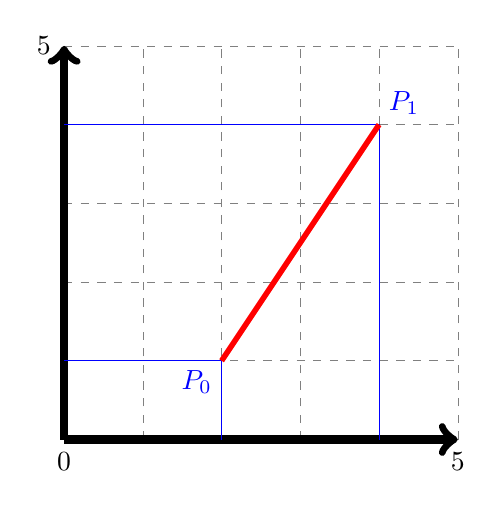
\begin{tikzpicture}
\draw[help lines, style=dashed] (0,0) grid (5,5);
\draw[->, line width = 3pt] (0,0) [below] node {0} -- (0,5) [left] node {5} ;
\draw[->, line width = 3pt] (0,0) -- (5,0) [below] node {5};
\draw[blue] (0,1) -- (2,1) [below left] node {$P_0$} -- (2,0);
\draw[blue] (0,4) -- (4,4) [above right] node {$P_1$} -- (4,0);
\draw[red, line width = 2pt] (2,1) -- (4,4);
\end{tikzpicture}
\end{center}
Given the two points of $P_0 (2,1)$ and $P_1 (4,4)$, the red line is the linear interpolant between the points. The linear interpolant  $L$ between two general points $P_0 = (x_0,y_0)$ and $P_1 (x_1,y_1)$ is computed by the equations \ref{eqnLinearInter1} or \ref{eqnLinearInter2}.
\begin{equation} \label{eqnLinearInter1}
\frac{y-y_0}{x-x_0} = \frac{y_1-y_0}{x_1-x_0} 
\end{equation}
\begin{equation} \label{eqnLinearInter2}
\mathbf {L} (t)=\mathbf {P} _{0}+t(\mathbf {P} _{1}-\mathbf {P} _{0})=(1-t)\mathbf {P} _{0}+t\mathbf {P} _{1}{\mbox{ , }}0\leq t\leq 1
\end{equation}
\end{note}

\begin{note}[Bézier curve]

A Bézier curve is a parametric curve frequently used in computer graphics and related fields. In vector graphics, Bézier curves are used to model smooth curves that can be scaled indefinitely. ``Paths", as they are commonly referred to in image manipulation programs, are combinations of linked Bézier curves.

A Bézier curve is defined by a set of control points $P_0$ through $P_n$, where $n$ is called its order (n = 1 for linear, 2 for quadratic, etc.). The first and last control points are always the end points of the curve; however, the intermediate control points (if any) generally do not lie on the curve.
\begin{itemize}
\item Linear Bézier curves:
Given points P0 and P1, a linear Bézier curve is simply a straight line between those two points. The curve is given by\\
\begin{equation}
\mathbf {B} (t)=\mathbf {P} _{0}+t(\mathbf {P} _{1}-\mathbf {P} _{0})=(1-t)\mathbf {P} _{0}+t\mathbf {P} _{1}{\mbox{ , }}0\leq t\leq 1
\end{equation}
and is equivalent to linear interpolation.
\item Quadratic Bézier curves:
A quadratic Bézier curve is the path traced by the function B(t), given points P0, P1, and P2,
\begin{equation}
\mathbf {B} (t)=(1-t)[(1-t)\mathbf {P} _{0}+t\mathbf {P} _{1}]+t[(1-t)\mathbf {P} _{1}+t\mathbf {P} _{2}]{\mbox{ , }}0\leq t\leq 1
\end{equation} ,which can be interpreted as the linear interpolant of corresponding points on the linear Bézier curves from P0 to P1 and from P1 to P2 respectively. Rearranging the preceding equation yields:
\begin{equation}
\mathbf {B} (t)=(1-t)^{2}\mathbf {P} _{0}+2(1-t)t\mathbf {P} _{1}+t^{2}\mathbf {P} _{2}{\mbox{ , }}0\leq t\leq 1.
\end{equation}
The derivative of the Bézier curve with respect to t is
\begin{equation}
\mathbf {B} '(t)=2(1-t)(\mathbf {P} _{1}-\mathbf {P} _{0})+2t(\mathbf {P} _{2}-\mathbf {P} _{1})\,.
\end{equation} 
from which it can be concluded that the tangents to the curve at P0 and P2 intersect at P1. As t increases from 0 to 1, the curve departs from P0 in the direction of P1, then bends to arrive at P2 from the direction of P1.
The second derivative of the Bézier curve with respect to t is
\begin{equation}
\mathbf {B} ''(t)=2(\mathbf {P} _{2}-2\mathbf {P} _{1}+\mathbf {P} _{0})
\end{equation}

\begin{center}
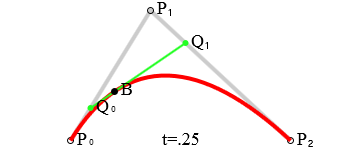
\includegraphics[scale=0.8]{Images/etc/bei}
\end{center}


\end{itemize}


\end{note}
\end{document}